
\documentclass{article} % For LaTeX2e
\usepackage{iclr2026_conference,times}
\usepackage{graphicx}
\usepackage{amsmath}
\usepackage{amssymb}

\usepackage{amsmath,amssymb,amsthm,mathtools}
\usepackage{bm}
\usepackage{enumitem}
\usepackage[colorlinks=true,linkcolor=blue,citecolor=blue]{hyperref}
\theoremstyle{plain}
\newtheorem{theorem}{Theorem}
\newtheorem{conjecture}{Conjecture}
\newtheorem{proposition}{Proposition}
\newtheorem{lemma}{Lemma}
\newtheorem{corollary}{Corollary}
\theoremstyle{definition}
\newtheorem{assumption}{Assumption}
\newtheorem{definition}{Definition}
\newtheorem{remark}{Remark}
 
\newcommand{\R}{\mathbb{R}}
\newcommand{\E}{\mathbb{E}}
\newcommand{\Var}{\operatorname{Var}}
\newcommand{\sgn}{\operatorname{sign}}
\newcommand{\Fmap}{F}
\newcommand{\xbar}{\bar{x}}
\DeclareMathOperator*{\argmin}{arg\,min}
\newcommand{\Cov}{\operatorname{Cov}}
\newcommand{\ybar}{\bar{y}}
\newcommand{\ytil}{\tilde{y}}
\newcommand{\half}{\tfrac12}
\DeclarePairedDelimiter{\paren}{(}{)}
\newcommand{\norm}[1]{\left\lVert #1\right\rVert}
\newcommand{\pp}{p_{+}}
\newcommand{\pmm}{p_{-}}
% Optional math commands from https://github.com/goodfeli/dlbook_notation.
\input{math_commands.tex}

\usepackage{hyperref}
\usepackage{url}
\usepackage{xcolor}
\newcommand{\pier}[1]{{\color{red} Pier: #1}}



\title{}

% Authors must not appear in the submitted version. They should be hidden
% as long as the \iclrfinalcopy macro remains commented out below.
% Non-anonymous submissions will be rejected without review.

\author{Antiquus S.~Hippocampus, Natalia Cerebro \& Amelie P. Amygdale \thanks{ Use footnote for providing further information
about author (webpage, alternative address)---\emph{not} for acknowledging
funding agencies.  Funding acknowledgements go at the end of the paper.} \\
Department of Computer Science\\
Cranberry-Lemon University\\
Pittsburgh, PA 15213, USA \\
\texttt{\{hippo,brain,jen\}@cs.cranberry-lemon.edu} \\
\And
Ji Q. Ren \& Yevgeny LeNet \\
Department of Computational Neuroscience \\
University of the Witwatersrand \\
Joburg, South Africa \\
\texttt{\{robot,net\}@wits.ac.za} \\
\AND
Coauthor \\
Affiliation \\
Address \\
\texttt{email}
}

% The \author macro works with any number of authors. There are two commands
% used to separate the names and addresses of multiple authors: \And and \AND.
%
% Using \And between authors leaves it to \LaTeX{} to determine where to break
% the lines. Using \AND forces a linebreak at that point. So, if \LaTeX{}
% puts 3 of 4 authors names on the first line, and the last on the second
% line, try using \AND instead of \And before the third author name.

\newcommand{\fix}{\marginpar{FIX}}
\newcommand{\new}{\marginpar{NEW}}

%\iclrfinalcopy % Uncomment for camera-ready version, but NOT for submission.
\begin{document}


\maketitle

\begin{abstract}
Deep neural networks trained with finite-step-size stochastic gradient descent are widely observed to operate near an \textit{edge of stochastic stability}. Understanding their stabilization dynamics is difficult for two reasons. First, even on a quadratic loss, mini-batch randomness separates several notions of stability, making it unclear which edge governs the observed behavior. Second, even beyond the relevant edge, the quadratic model is unstable and therefore cannot explain why training remains bounded. We identify the \textit{harmonic edge} as the threshold governing the distributional transition studied here. Training progressively sharpens toward this edge, briefly crosses it, and is pushed back by higher-order terms into a self-stabilized state. Harmonic instability creates depletion around the solution. We characterize these conditions and validate the resulting dynamics in stochastic models, matrix factorization, and deep neural networks.

\end{abstract}

% {\color{red}Hey Avrajit, this is Marc. I haven't had access to the slack channel in the past week! If you need to reach me for something: 4244135035 or marcwalden@g.harvard.edu}

\section{Introduction}
\paragraph{Gradient descent at the edge of stability and self-stabilization}

\paragraph{Correct edge for SGD is the instable one.}


\paragraph{Instability threshold for SGD on quadratic is based on moment}


% Let \(L:\mathbb R^d\to \mathbb R\) be a \(C^5\) loss and let $x^\star$ be a local minimizer.  We consider stochastic-gradient dynamics
% \begin{equation}
%     X_{t+1}=X_t-\eta\,g(X_t;\xi_t),
%     \qquad \E_{\xi}[g(x;\xi)]=\nabla L(x),
%     \label{eq:sgd}
% \end{equation}
% where $\eta>0$ is the step size and $\xi_t$ denotes the sampled mini-batch or stochastic-gradient randomness. Expanding a stochastic gradient around $x^\star$ gives
% \begin{equation}
%  g(x^\star+\Delta;\xi)
%  =g(x^\star;\xi)+H_{\xi}\Delta+N_{\xi}(\Delta),
%  \qquad N_{\xi}(\Delta)=O(\norm{\Delta}^2),
%  \label{eq:localgrad}
% \end{equation}
% with stochastic curvature $H_{\xi}=\nabla_xg(x^\star;\xi)$.  Hence the local recursion is
% \begin{equation}
%  \Delta_{t+1}
%  =A_t\Delta_t+\zeta_t+R_t(\Delta_t),
%  \qquad
%  A_t=I-\eta H_{\xi_t},
%  \quad
%  \zeta_t=-\eta g(x^\star;\xi_t),
%  \label{eq:localnormal}
% \end{equation}
% where $R_t(\Delta)=-\eta N_{\xi_t}(\Delta)$.  Equation~\eqref{eq:localnormal} separates three mechanisms:
% \begin{enumerate}[leftmargin=1.6em,itemsep=0.15em]
%     \item the random linear cocycle $A_t$, which determines linear stochastic stability;
%     \item the additive residual $\zeta_t$, which may vanish in interpolating problems and is Gaussian only in the additive-noise specialization;
%     \item the higher order $R_t$ responsible for self-stabilization and bimodality.
% \end{enumerate}
% %  For full-batch gradient descent, local stability is controlled by the eigenvalues of one fixed Jacobian.  For SGD, the Jacobian changes with the sampled batch, and the relevant object is the product
% % \begin{equation}
% %  A_{t-1}A_{t-2}\cdots A_0.
% % \end{equation}
% % Different functionals of this random product produce different critical step sizes.  Mean-square stability controls the second moment, whereas the top Lyapunov exponent controls the growth of a typical infinitesimal perturbation.  Rare curvature samples can destabilize the second moment long before they destabilize a typical trajectory.  Thus moment blow-up, pathwise instability, and bimodality are distinct transitions.

% For example in a scalar loss $ \ell_h(x)=\frac{h}{2}x^2-\frac{\alpha}{4}x^4+\frac{\beta}{6}x^6,
%  \quad (\alpha,\beta)>0$ with sub-quartic behaviour, the iterates yield:
% \begin{equation}
%  X_{t+1}=(1-\eta h_t)X_t+\eta\alpha X_t^3-\eta\beta X_t^5+\zeta_t.
%  \label{eq:polynomialsgd}
% \end{equation}
% Unlike deterministic GD, SGD admits multiple inequivalent notions of local stability, depending on which moment of the linearized iterates is controlled. We begin with the general notion of positive q-moment stability.

% For every $q>0$, the linear stochastic recursion satisfies
% \begin{equation}
%     \mathbb{E}_{h_t}\left[|X_t|^q\right]
%     =
%     |X_0|^q
%     \left(
%         \mathbb{E}_{h_t}\left[|1-\eta h_t|^q\right]
%     \right)^t,
% \end{equation}
% so the stability of the $q$-th moment is determined by
% $\mathbb{E}_{h}[|1-\eta h_t|^q]$. This motivates the following definition.
% \begin{definition}[$q$-moment stability]
% For $q>0$, 
% The origin is $q$-moment stable when $\mathbb{E}_{h_{t}}[|1-\eta h_t|^q]<1$, and the corresponding edge $\eta_q$ solves $m_q(\eta_q)=1$.
% \end{definition}

% The case $q=2$ corresponds to mean-square stability, while $q=1$ corresponds to absolute first-moment stability. The pathwise stability criterion is obtained in the limit $q\to 0$, since
% \begin{equation}
%     \lim_{q\to 0}\frac{1}{q}\log m_q(\eta)
%     =
%     \mathbb{E}\!\left[\log |1-\eta h|\right]
%     =: \lambda(\eta),
% \end{equation}
% under the integrability condition
% $\mathbb{E}[|\log |1-\eta h||]<\infty$.
% The origin is Lyapunov stable when $\lambda(\eta)<0$, and the corresponding Lyapunov edge $\eta_{\mathrm{L}}$ satisfies
% \begin{equation}
%     \mathbb{E}\!\left[\log |1-\eta_{\mathrm{L}}h|\right]=0.
% \end{equation}

% \begin{proposition}[Moment hierarchy]
% If $q_2>q_1>0$ and $m_{q_2}(\eta)<1$, then $m_{q_1}(\eta)<1$.  In particular,
% \begin{equation}
%     \text{mean-square stable}
%     \Longrightarrow
%     \text{absolute-mean stable}
%     \Longrightarrow
%     \text{Lyapunov stable}.
%     \label{eq:hierarchy}
% \end{equation}
% \end{proposition}


\paragraph{Background: Exact stability threshold for scalar stochastic quadratic}
\label{sec:exact-scalar-gain}

Consider the scalar stochastic-quadratic recursion
\(x_{t+1}=(1-\eta h_t)x_t\), where \((h_t)_{t\geq0}\) are i.i.d. copies
of a nonnegative random curvature \(h\). Set
\(G_\eta:=|1-\eta h|\),
\(m_q(\eta):=\mathbb{E}[G_\eta^q]\) for \(q>0\),
\(\lambda(\eta):=\mathbb{E}[\log G_\eta]\), and
\(r_\alpha(\eta):=\mathbb{E}[G_\eta^{-\alpha}]\) for \(\alpha>0\).
Here \(m_q\) measures positive-moment growth, \(\lambda\) is the
pathwise Lyapunov exponent, and \(r_\alpha\) measures inverse-moment
growth near the origin. Whenever \(r_\alpha\) is used, we assume
\(\mathbb{P}(G_\eta=0)=0\) and \(r_\alpha(\eta)<\infty\).

\begin{theorem}[Exact stochastic-quadratic gain law]
\label{thm:exact-scalar-gain}
Let \(x_0\neq0\). Then
\(x_n=x_0\prod_{t=0}^{n-1}(1-\eta h_t)\), and consequently
\(\mathbb{E}|x_n|^q=|x_0|^q m_q(\eta)^n\) for every \(q>0\), while
\(\mathbb{E}|x_n|^{-\alpha}
=|x_0|^{-\alpha}r_\alpha(\eta)^n\) whenever the latter expectation is
finite. Moreover, if \(\mathbb{E}|\log G_\eta|<\infty\), then
\(n^{-1}\log(|x_n|/|x_0|)\to\lambda(\eta)\) almost surely.

Therefore, \(m_q(\eta)<1\) is equivalent to exponential \(q\)-moment
stability, \(\lambda(\eta)<0\) is equivalent to pathwise exponential
stability, and \(r_\alpha(\eta)<1\) gives exponential inverse-moment
anti-concentration away from the origin. Their respective boundaries
are \(m_q(\eta)=1\), \(\lambda(\eta)=0\), and \(r_\alpha(\eta)=1\).
Furthermore,
\[
r_\alpha(\eta)<1
\quad\Longrightarrow\quad
\lambda(\eta)>0
\quad\Longrightarrow\quad
m_q(\eta)>1
\qquad\text{for every }q>0.
\]
If \(q_2>q_1>0\), then \(m_{q_2}(\eta)<1\) implies
\(m_{q_1}(\eta)<1\).
\end{theorem}
\begin{proof}
The product representation follows by iterating the recursion, and
independence gives the two moment identities. The almost-sure limit
follows from the strong law of large numbers applied to
\(\log G_{\eta,t}\). Jensen's inequality gives
\(-\alpha\lambda(\eta)\leq\log r_\alpha(\eta)\), so
\(r_\alpha(\eta)<1\) implies \(\lambda(\eta)>0\). Similarly,
\(\log m_q(\eta)\geq q\lambda(\eta)\), so
\(\lambda(\eta)>0\) implies \(m_q(\eta)>1\). The final implication
follows from Lyapunov's moment inequality.
\end{proof}


\begin{figure}
    \centering
    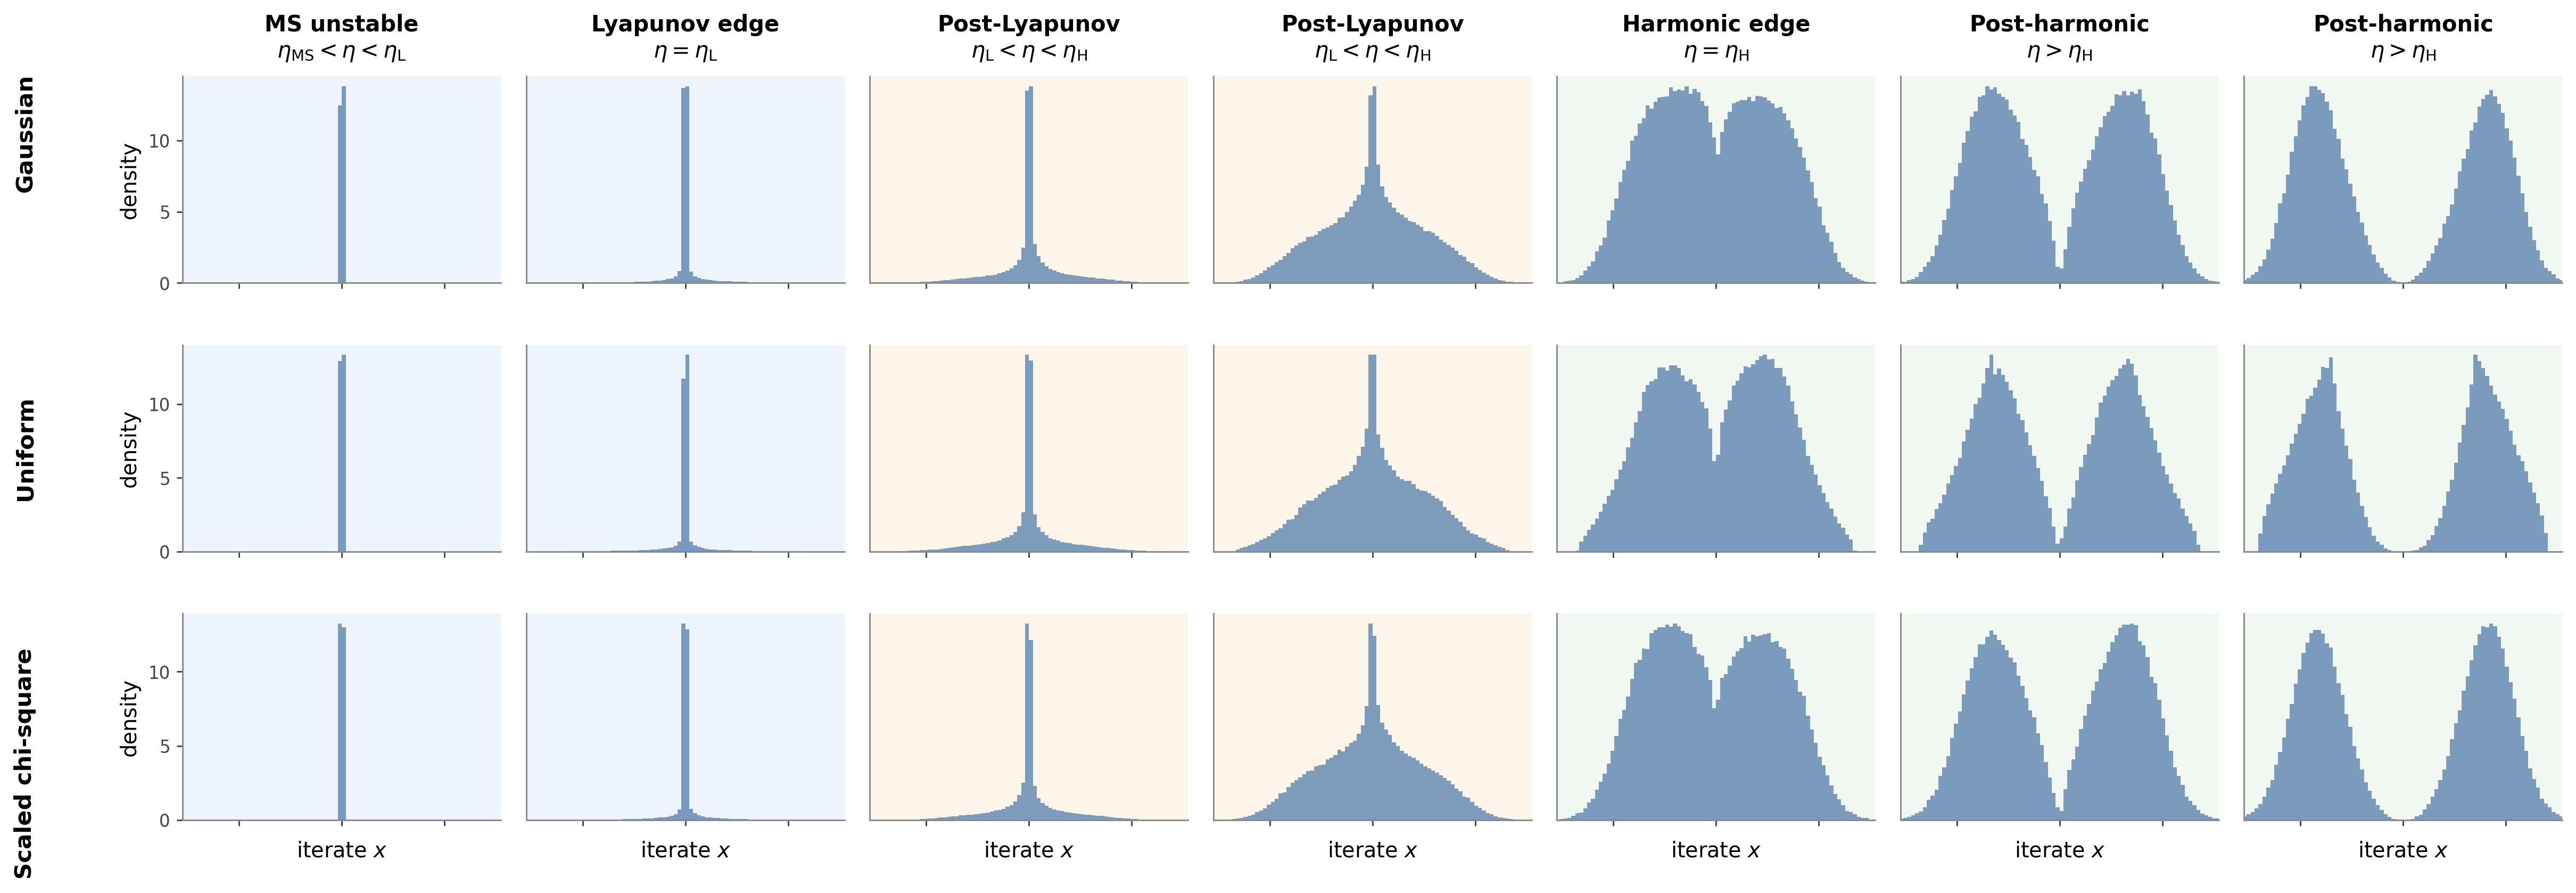
\includegraphics[width=1.0\linewidth]{img/continuous_curvature_histograms_raw_scientific_with_variable_regimes.png}
    \caption{Evolution of the quasi-stationary iterate distribution across stochastic-stability regimes for Gaussian, uniform, and scaled chi-square curvature with matched mean and variance. Between the mean-square and Lyapunov edges, $\eta_{\mathrm{MS}}<\eta<\eta_{\mathrm{L}}$, the second moment is unstable while the distribution remains sharply concentrated near the origin. Beyond the Lyapunov edge, $\eta>\eta_{\mathrm{L}}$, the central peak broadens, and near the empirical harmonic threshold $\widehat{\eta}_{\mathrm{H}}$ the distribution develops two separated lobes. For $\eta>\widehat{\eta}_{\mathrm{H}}$, central depletion becomes pronounced and a clear bimodal state emerges.}
\end{figure}

\paragraph{Deterministic versus random curvature.}
If \(h_t\equiv\bar h>0\), then \(G_\eta=|1-\eta\bar h|\), and all three
nontrivial boundaries reduce to \(G_\eta=1\), equivalently
\(\eta=2/\bar h\). Thus positive-moment, Lyapunov, and inverse-moment
thresholds coincide for deterministic curvature. For random curvature,
define the log-moment function
\(\Psi_\eta(s):=\log\mathbb{E}[G_\eta^s]\). Then
\(\Psi_\eta(q)=\log m_q(\eta)\),
\(\Psi_\eta'(0)=\lambda(\eta)\), and
\(\Psi_\eta(-\alpha)=\log r_\alpha(\eta)\). Since
\(\Psi_\eta\) is generally strictly convex when \(G_\eta\) is
nonconstant, the three thresholds need not coincide.


\begin{theorem}[Restated]
\label{thm:quadratic-sgd-kesten}
Let $(B_t)_{t\geq 0}$ be i.i.d., with each batch defining the exact
quadratic loss
\[
L_B(\mathbf{u})
=
\frac{1}{2}\mathbf{u}^{\top}\mathbf{H}_B\mathbf{u}
-
\boldsymbol{\xi}_B^{\top}\mathbf{u},
\qquad
\mathbf{H}_B\succeq\mathbf{0},
\qquad
\mathbb{E}[\boldsymbol{\xi}_B]=\mathbf{0}.
\]
Constant-step-size SGD obeys
\[
\mathbf{u}_{t+1}
=
(\mathbf{I}-\eta\mathbf{H}_{B_t})\mathbf{u}_t
+
\eta\boldsymbol{\xi}_{B_t}.
\]
Defining the linear multiplier product as $\mathbf{A}_B:=\mathbf{I}-\eta\mathbf{H}_B$, the multiplier
product $\boldsymbol{\Pi}_n:=(\mathbf{I}-\eta\mathbf{H}_{B_{n-1}})\cdots
(\mathbf{I}-\eta\mathbf{H}_{B_{0}})$, the almost-sure top Lyapunov exponent
$\gamma_\eta:=\lim_{n\to\infty}n^{-1}\log\|\boldsymbol{\Pi}_n\|$,
and the moment growth function
$k_\eta(s):=\lim_{n\to\infty}
\bigl(\mathbb{E}\|\boldsymbol{\Pi}_n\|^s\bigr)^{1/n}$. Further assuming that:
\begin{enumerate}
\item The linear dynamics are contractive on average $\gamma_\eta<0$. 
\item There exists a tail exponent $\kappa_\eta>0$ satisfying $k_\eta(\kappa_\eta)=1$
\item The matrices $\mathbf{A}_B$ satisfy the standard multivariate
    Kesten conditions: they are invertible almost surely, their support is strongly irreducible and proximal,
    and the associated multiplicative process is non-arithmetic.

    \item For some $\varepsilon>0$, $    \mathbb{E}\|\mathbf{A}_B\|^{\kappa_\eta+\varepsilon}
    +
    \mathbb{E}\|\boldsymbol{\xi}_B\|^{\kappa_\eta+\varepsilon}
    <\infty$ and the affine recursion has no common deterministic fixed point:
    for every $\mathbf{x}\in\mathbb{R}^d$, $    \mathbb{P}\!\left(
    \mathbf{A}_B\mathbf{x}+\eta\boldsymbol{\xi}_B=\mathbf{x}
    \right)<1.$
\end{enumerate}

Then the recursion admits a unique stationary distribution. If
$\mathbf{u}_\eta$ follows this distribution, then
\[
\mathbb{P}\!\left(\|\mathbf{u}_\eta\|>t\right)
\sim C_\eta t^{-\kappa_\eta},
\qquad t\to\infty,
\]
where $C_\eta>0$. Moreover, for every nondegenerate direction $\mathbb{P}\!\left(
|\mathbf{v}^{\top}\mathbf{u}_\eta|>t
\right)
\sim
C_\eta(\mathbf{v})t^{-\kappa_\eta},
\qquad t\to\infty$.
\end{theorem}
\begin{figure}
    \centering
    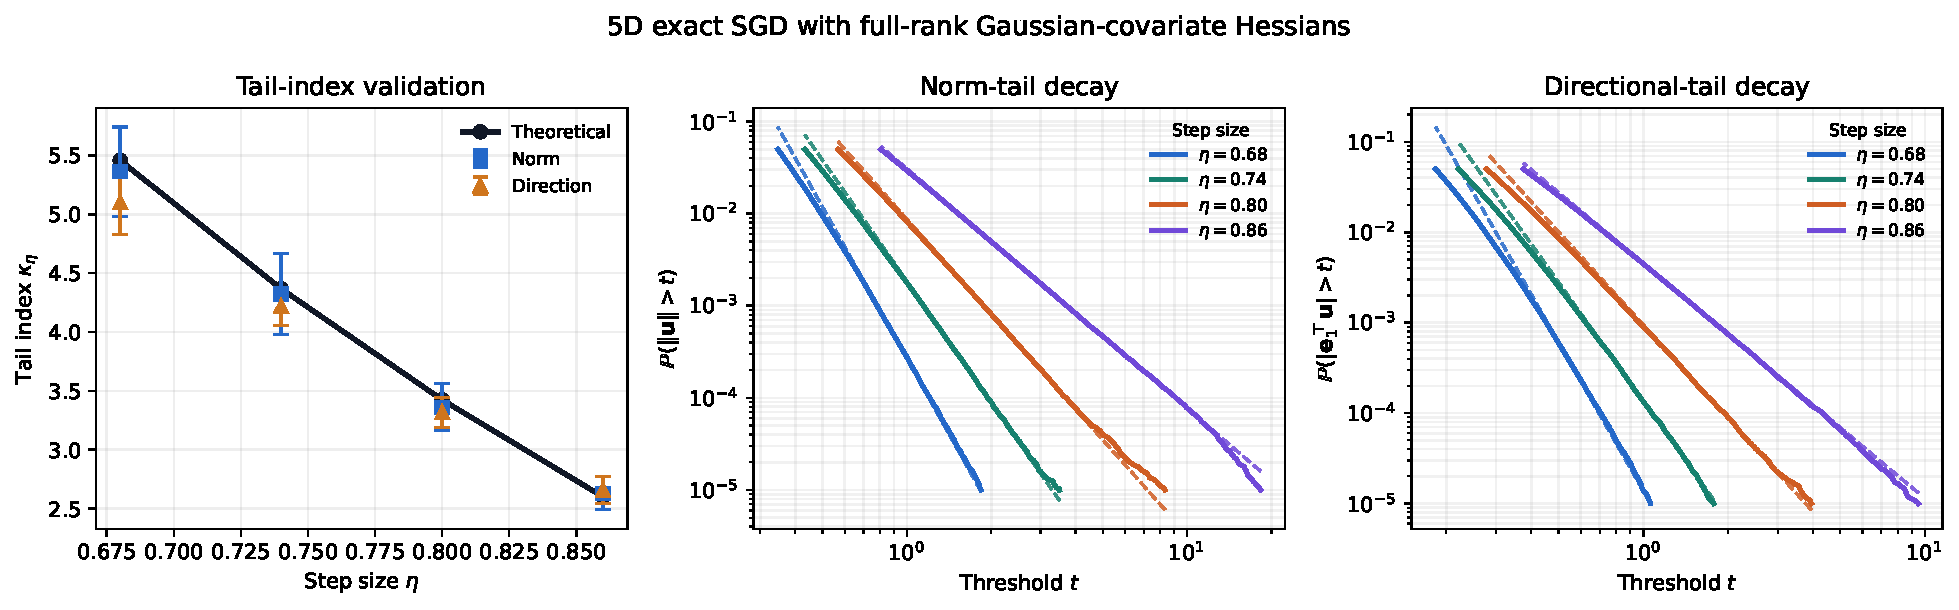
\includegraphics[width=0.9\linewidth]{img/figure_covariate_tail_validation.pdf}
\caption{Kesten-tail for linear regression with Gaussian-covariate. Left: theoretical and empirical tail indices. Center and right: empirical norm and directional tails (solid) with predicted slopes $-\kappa_\eta$ (dashed). Both observables share the predicted exponent, which decreases as the step size increases.}

    \label{fig:kesten-valid}
\end{figure}

\paragraph{Validation on Linear Regression with Batch sampled Covariates.}
To verify that the observed power law, we repeat the experiment using exact mini-batch linear-regression
losses.  For each batch, let
$\mathbf X_B\in\mathbb R^{5\times 5}$ have i.i.d. $\mathcal N(0,1)$ entries and
let $\boldsymbol\varepsilon_B\sim
\mathcal N(\mathbf 0,0.08^2\,5\,\mathbf I)$.  We use
\[
L_B(\mathbf u)
=\frac{1}{2\cdot 5}\|\mathbf X_B\mathbf u-
\boldsymbol\varepsilon_B\|^2,
\qquad
\mathbf H_B=\frac{1}{5}\mathbf X_B^\top\mathbf X_B,
\qquad
\boldsymbol\xi_B=\frac{1}{5}\mathbf X_B^\top
\boldsymbol\varepsilon_B.
\]
Thus $\mathbf H_B$ is a full-rank Wishart matrix almost surely, and
SGD obeys the exact affine recursion
$\mathbf u_{t+1}=(\mathbf I-\eta\mathbf H_{B_t})\mathbf u_t+
\eta\boldsymbol\xi_{B_t}$.  Orthogonal invariance of the Wishart law implies
that the product equals the one-step 
$k_\eta(s)=\mathbb E\|(\mathbf I-\eta\mathbf H_B)\mathbf e_1\|^s$. Although the Kesten exponent is defined through the full product,
orthogonal invariance of the Gaussian Wishart law implies
\[
k_\eta(s)
=
\lim_{n\to\infty}
\left(\mathbb E\|\boldsymbol{\Pi}_n\|^s\right)^{1/n}
=
\mathbb E\|(\mathbf I-\eta\mathbf H_B)\mathbf e_1\|^s.
\]
Thus, in this isotropic setting only, the product can be evaluated
from a one-step moment.
More explicitly, if $R\sim\chi^2_5$ and $Q\sim\chi^2_4$ are independent, then
\[
\|(\mathbf I-\eta\mathbf H_B)\mathbf e_1\|^2
=\left(1-\frac{\eta R}{5}\right)^2+\frac{\eta^2RQ}{25},
\]
which we evaluate by Gauss--Laguerre quadrature.  For each step size we use
eight independent chains, discard $10^5$ burn-in iterations, and retain
$6\times10^5$ iterates per chain.



The theoretical and empirical tail indices are
\[
\begin{array}{c|cccc}
\eta & 0.68 & 0.74 & 0.80 & 0.86\\ \hline
\kappa_\eta\ \text{(theory)} & 5.457 & 4.367 & 3.425 & 2.601\\
\widehat\kappa_{\|\mathbf u\|} & 5.361 & 4.322 & 3.361 & 2.631\\
\widehat\kappa_{|\mathbf e_1^\top\mathbf u|}
& 5.101 & 4.218 & 3.318 & 2.657
\end{array}
\]
and the top Lyapunov exponent is negative at every tested step size.  An
independent Monte Carlo check with two million fresh full covariate matrices
also gives
$\mathbb E\|(\mathbf I-\eta\mathbf H_B)\mathbf e_1\|^{\kappa_\eta}
\approx 1$ at all four pressure roots.


\paragraph{Negative moments and anti-concentration near the origin}

The condition $r_\alpha(\eta)=\mathbb{E}[G_\eta^{-\alpha}]<1$ has a direct
finite-time meaning. It certifies that the linear dynamics make
returns toward the origin exponentially unlikely.

\begin{proposition}[Finite-time anti-concentration]
\label{prop:anti-concentration}
Suppose $x_0\neq0$ and $r_\alpha(\eta)<1$ for some $\alpha>0$. Then, for every
$\varepsilon>0$ and $n\geq1$,
\[
\mathbb{P}\!\left(|x_n|\leq\varepsilon\,\middle|\,x_0\right)
\leq
\left(\frac{\varepsilon}{|x_0|}\right)^\alpha r_\alpha(\eta)^n.
\]
Consequently, for every $T\geq1$,
$\mathbb{P}(\min_{1\leq n\leq T}|x_n|\leq\varepsilon\mid x_0)
\leq(\varepsilon/|x_0|)^\alpha
\sum_{n=1}^{T}r_\alpha(\eta)^n
\leq(\varepsilon/|x_0|)^\alpha r_\alpha(\eta)/(1-r_\alpha(\eta))$.
\end{proposition}

\begin{proof}
By Markov's inequality and Theorem~\ref{thm:exact-scalar-gain},
\[
\mathbb{P}(|x_n|\leq\varepsilon\mid x_0)
=
\mathbb{P}(|x_n|^{-\alpha}\geq\varepsilon^{-\alpha}\mid x_0)
\leq
\varepsilon^\alpha\mathbb{E}[|x_n|^{-\alpha}\mid x_0]
=
\left(\frac{\varepsilon}{|x_0|}\right)^\alpha r_\alpha(\eta)^n.
\]
The finite-horizon statement follows from the union bound and the geometric
series.
\end{proof}

Thus $r_\alpha(\eta)<1$ gives inverse-moment anti-concentration near the
origin. As established in Theorem~\ref{thm:exact-scalar-gain},
\[
r_\alpha(\eta)<1
\quad\Longrightarrow\quad
\lambda(\eta)>0
\quad\Longrightarrow\quad
m_q(\eta)>1
\qquad\text{for every }q>0.
\]
For a nonlinear recurrent system, this local repulsion can lead to central
depletion only when combined with global confinement and a sufficiently
regular reinjection mechanism.

\paragraph{The harmonic case.}
The choice $\alpha=1$ gives the harmonic moment
$r_1(\eta)=\mathbb{E}[G_\eta^{-1}]$. Its boundary $r_1(\eta)=1$ is meaningful
only when this expectation is finite. For a finite discrete curvature distribution,
$r_1(\eta)<\infty$ provided that no curvature value satisfies $h=1/\eta$.
If $\mathbb{P}(h=1/\eta)>0$, then $\mathbb{P}(G_\eta=0)>0$ and every negative
moment is infinite.

Suppose instead that $h$ has a continuous, locally bounded density that is
strictly positive near $1/\eta$. Then $G_\eta$ has a density that is positive
near zero, and hence $\mathbb{E}[G_\eta^{-\alpha}]<\infty$ for
$0<\alpha<1$, whereas $\mathbb{E}[G_\eta^{-\alpha}]=\infty$ for
$\alpha\geq1$. In particular, divergence of $r_1(\eta)$ does not certify
harmonic instability; it means that the literal harmonic criterion is not
well defined.

In this continuous setting, we therefore use fractional negative moments
with $0<\alpha<1$. For empirical diagnostics, we additionally report
truncated moments $\mathbb{E}[(G_\eta\vee\delta)^{-\alpha}]$ and small-gain
probabilities $\mathbb{P}(G_\eta\leq\delta)$ over several truncation levels
$\delta$. These truncated quantities are diagnostics only and do not satisfy
the exact product identity of Theorem~\ref{thm:exact-scalar-gain}.


\paragraph{Harmonic negative moments, central depletion, and bimodality}
\label{sec:harmonic-bimodality}

The harmonic condition controls the \emph{local behavior of the stationary
density at the origin}.  To make this distinction precise, consider the post-Lyapunov
scalar multiplier $M>0$, define
$r_{\alpha}(\eta):=\mathbb{E}[M^{-\alpha}]$, and let
$\alpha_{\eta}>0$ solve $r_{\alpha_{\eta}}(\eta)=1$.  Under the Cram\'er,
renewal-density, finite-cycle, and regular-reinjection assumptions of
Theorem~(yet to be added), the reflection-symmetric signed
coordinate $A$ satisfies
\begin{equation}
    p_A(a)\sim C_{\eta}|a|^{\alpha_{\eta}-1},
    \qquad a\to0,
    \label{eq:harmonic-local-density}
\end{equation}
for some $C_{\eta}>0$.  If
$s\mapsto\log\mathbb{E}[M^{-s}]$ is finite and strictly convex on an
interval containing $[0,\max\{1,\alpha_{\eta}\}]$, then
\begin{equation}
\begin{aligned}
 r_1(\eta)>1
 &\Longleftrightarrow 0<\alpha_{\eta}<1
 &&\Longrightarrow p_A(a)\to\infty,
 \\
 r_1(\eta)=1
 &\Longleftrightarrow \alpha_{\eta}=1
 &&\Longrightarrow p_A(a)\sim C_{\eta},
 \\
 r_1(\eta)<1
 &\Longleftrightarrow \alpha_{\eta}>1
 &&\Longrightarrow p_A(a)\to0.
\end{aligned}
\label{eq:harmonic-shape-trichotomy}
\end{equation}
Thus, on a parameter branch where $r_1(\eta)$ decreases through one, the
harmonic edge $\eta_{\mathrm H}$ defined by
$\mathbb{E}[M^{-1}]=1$ separates a central-cusp regime from an idealized
central-depletion regime.  In particular, between the Lyapunov and harmonic
edges the origin is pathwise repelling, yet rare contracting products can
still produce a divergent stationary cusp at the origin.

This conclusion is local.  Central depletion becomes exactly two spatial
modes only with additional global-shape assumptions.  For example, under
the hypotheses of Proposition~\ref{prop:mode-curvature}, if the projected
stationary density is even, tends to zero at infinity, has nonzero curvature
at the origin, and has at most one critical point on $(0,\infty)$, then
\begin{equation}
    p_A\text{ is bimodal}
    \quad\Longleftrightarrow\quad
    p_A''(0)>0.
    \label{eq:harmonic-bimodality-extra-shape}
\end{equation}
The restriction on positive critical points excludes shoulders, trimodality,
and competing outer modes.  A noisy period-two interpretation requires still
more: one-step sign reversal, contraction of the two-step return map, parity
predicting the occupied lobe, and noise smaller than the phase separation.
Consequently, the valid implication is
\begin{equation}
\begin{aligned}
 \text{post-harmonic local exponent}
 &\xrightarrow{\text{regular confinement/reinjection}}
 \text{central depletion},\\
 \text{central depletion}
 &\xrightarrow{\text{symmetry and global shape}}
 \text{two resolved lobes}.
\end{aligned}
 \label{eq:harmonic-implication-chain}
\end{equation}

\paragraph{Exact finite-step scalar experiment.}
We test these distinctions using ordinary discrete SGD.
Each batch $(h_t,\zeta_t)$ defines the smooth loss
\begin{equation}
 \ell_{h_t,\zeta_t}(x)
 =\frac12h_tx^2-\sigma\zeta_tx
 -\frac{\beta\rho}{2}\left[
 x^2-\rho\log\left(1+\frac{x^2}{\rho}\right)\right],
 \label{eq:harmonic-scalar-loss}
\end{equation}
and its exact constant-step update is
$x_{t+1}=(1-\eta h_t)x_t+
\eta\beta x_t^3/(1+x_t^2/\rho)+\eta\sigma\zeta_t$.
The linearized gain is $G_{\eta}=|1-\eta h|$, while the bounded nonlinear
term provides finite-amplitude confinement and vanishes to third order at
the origin.

We set $\mathbb{E}h=1$, $\operatorname{Var}(h)=0.04$, $\rho=1$,
$\beta=0.65$, $\sigma=0.003$, and
$\zeta\sim\operatorname{Unif}[-\sqrt{3},\sqrt{3}]$.  We compare three bounded
curvature laws with matched mean and variance: the two-point law
$h=1\pm0.2$; the uniform law
$h=1+\sqrt{3}(0.2)U$, $U\sim\operatorname{Unif}[-1,1]$; and the bounded
skewed law $h=0.66+0.8Y$,
$Y\sim\operatorname{Beta}(1.23675,1.67325)$.  On the tested step-size
interval, the gains are bounded away from zero, so the displayed negative
moments are finite.

For every curvature law we compute the mean-square edge
$\mathbb{E}G_{\eta}^{2}=1$, the Lyapunov edge
$\mathbb{E}\log G_{\eta}=0$, the fractional edge
$\mathbb{E}G_{\eta}^{-1/2}=1$, and the harmonic edge
$\mathbb{E}G_{\eta}^{-1}=1$.  The grid includes
$\varepsilon=0.01$ immediately before and after every candidate edge.  Four
independent seeds run $32$ chains per step size, discard $15{,}000$ updates,
and retain $20{,}000$ further updates per chain, storing every tenth state.

We distinguish three empirical quantities.  With a fixed Gaussian smoothing
bandwidth $b=0.02$, define
$C_b=b^2\widehat p_b''(0)/\widehat p_b(0)$.  The depletion edge
$\widehat\eta_{\mathrm{dep}}$ is the interpolated upward zero crossing of
$C_b$.  We declare two lobes resolved only when two consecutive grid points
satisfy
$\widehat p_b(0)/\max_{x>0}\widehat p_b(x)<0.8$ and the positive mode obeys
$\widehat x_{\star}>2b$.  The value $\widehat x_{\star}$ is reported
separately as the lobe location.  These are prespecified finite-noise,
finite-bandwidth definitions rather than universal population equivalences.

\begin{figure}
  \centering
  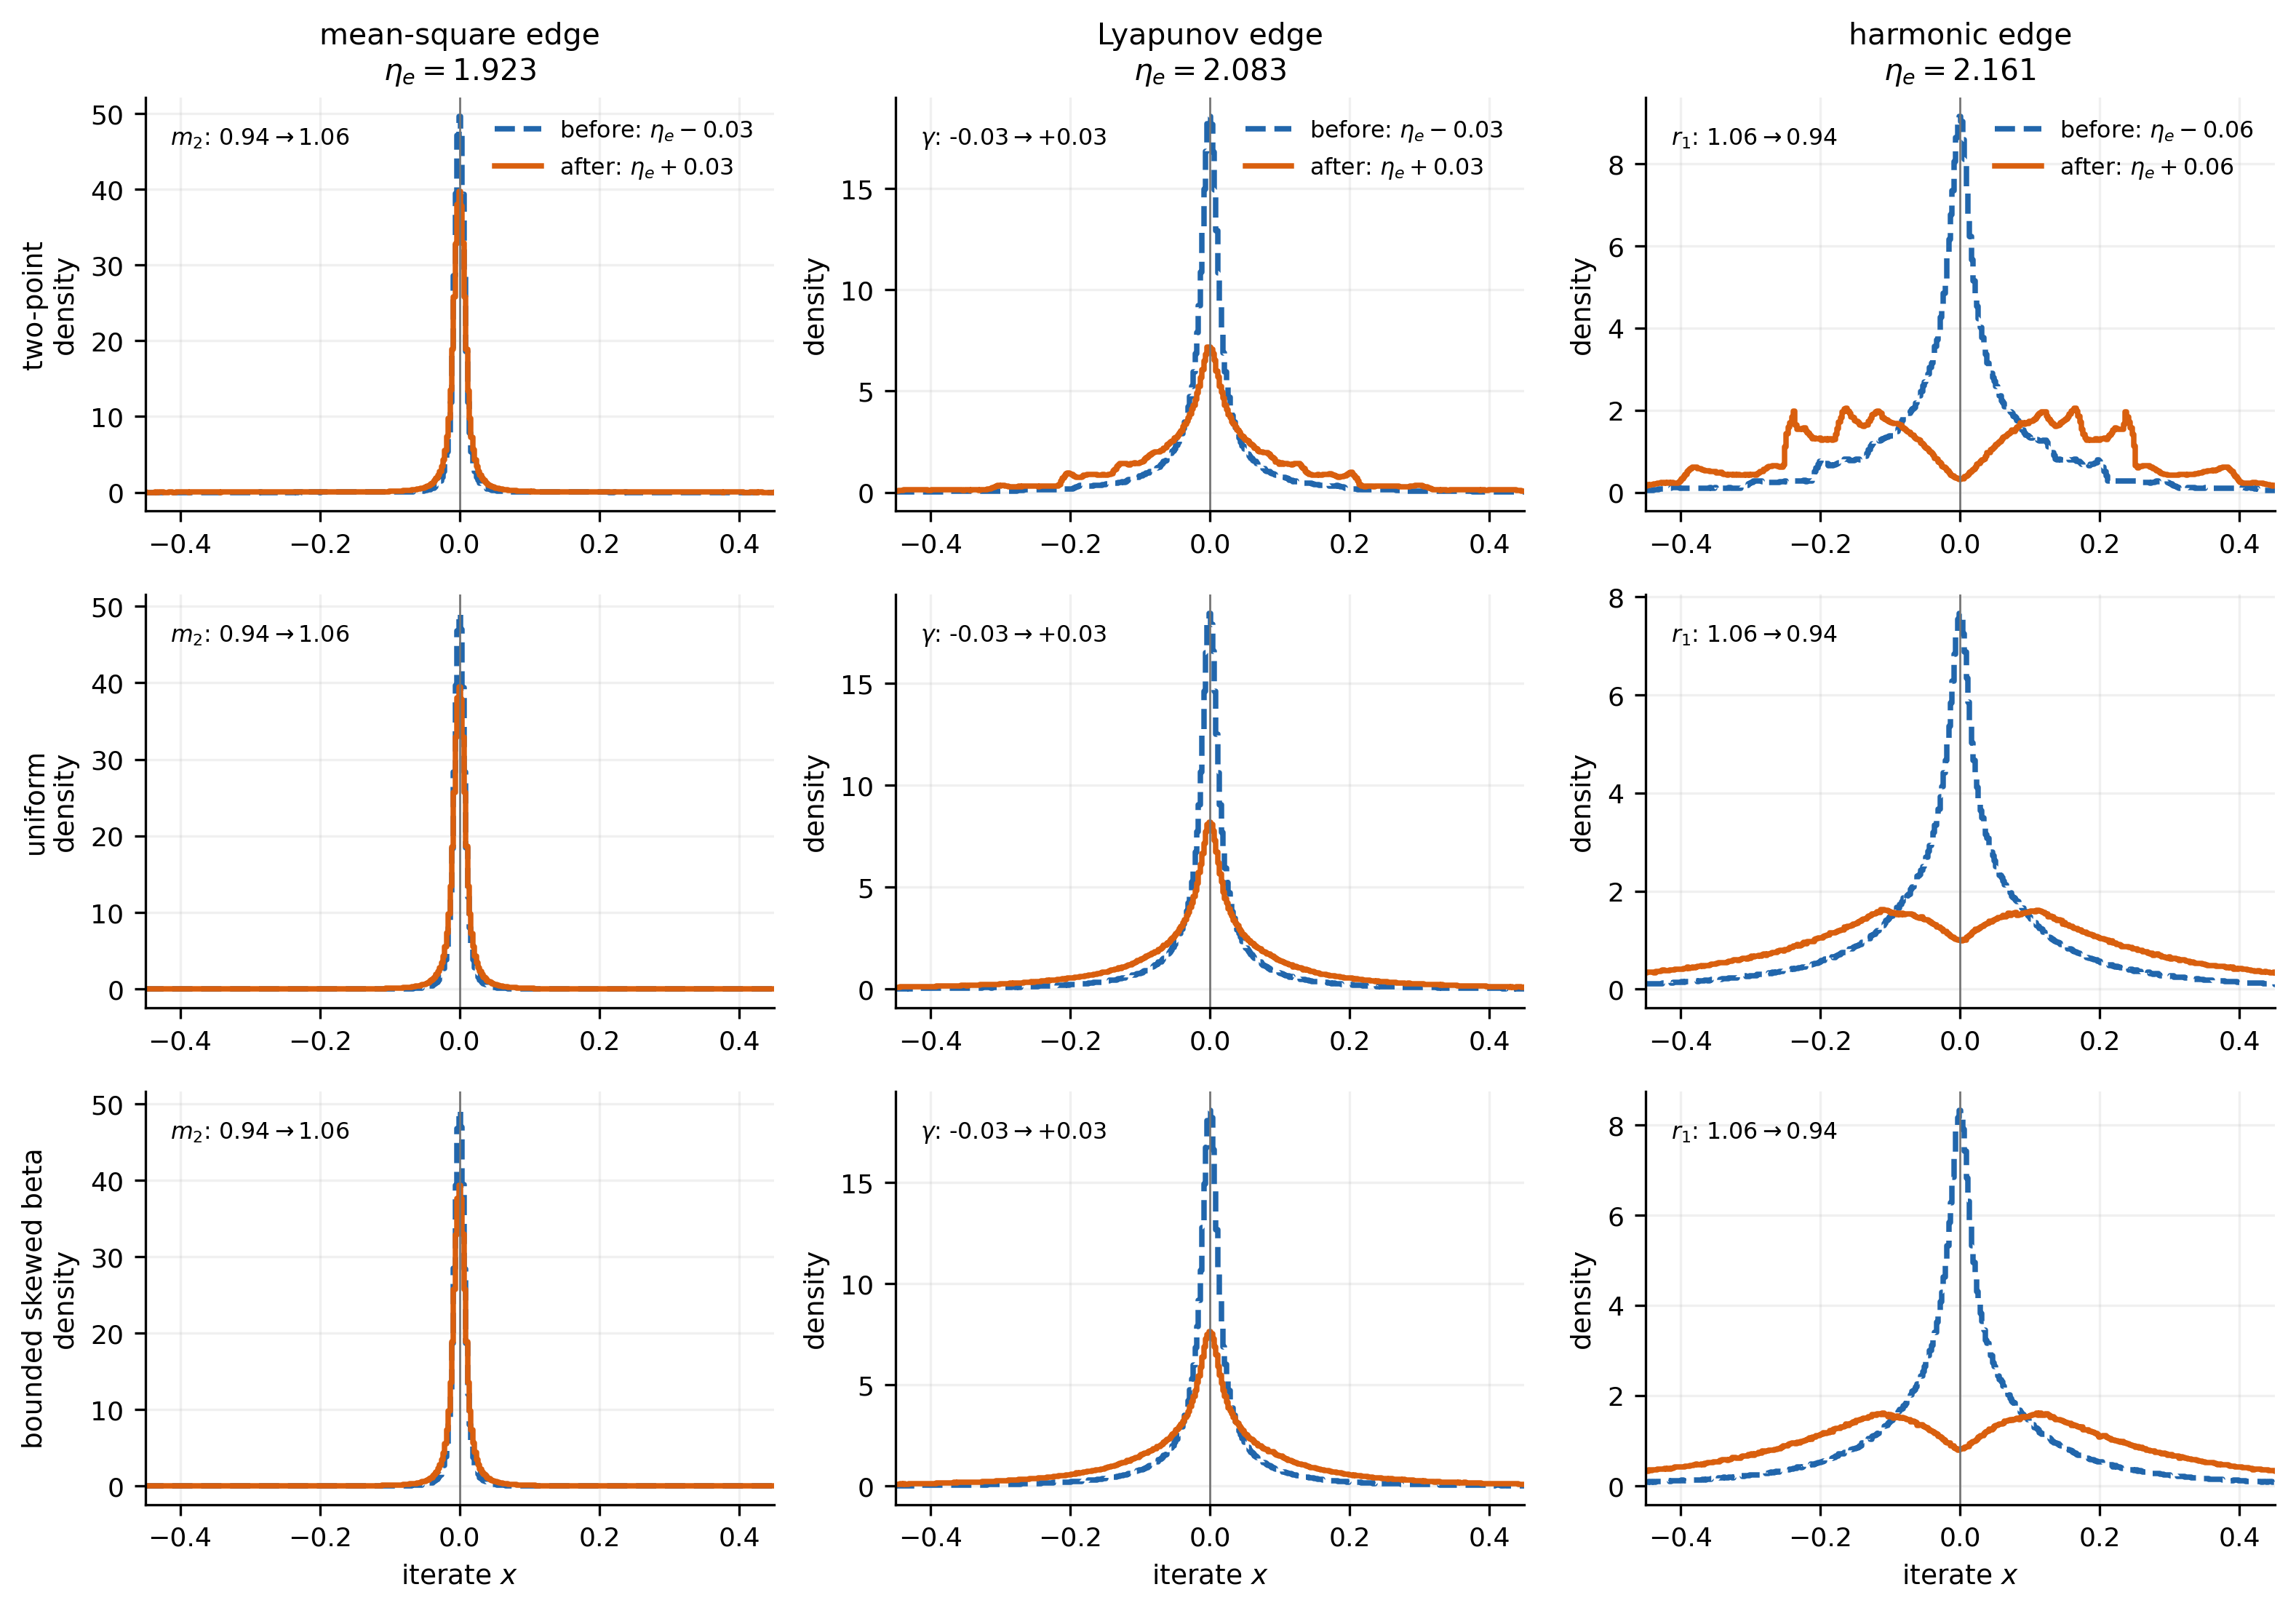
\includegraphics[width=\linewidth]{img/scalar_edge_transition_atlas.png}
  \caption{Exact discrete densities immediately before and after
  every candidate edge.}
  \label{fig:harmonic-edge-densities}
\end{figure}




Figure~\ref{fig:harmonic-edge-densities} shows the density at
$\varepsilon=0.01$ before and after each edge.  Crossing the mean-square edge
does not visibly change the sharp central peak.  At the Lyapunov edge the
density is broader but remains centrally peaked, and the same is true at the
fractional $\alpha=1/2$ edge.  The harmonic crossing is substantially closer
to the loss of central curvature.  Nevertheless, its offset from the
empirical depletion edge is law-dependent: $0.002$, $0.021$, and $0.013$ for
the two-point, uniform, and skewed laws.  Two resolved lobes appear a further
$0.018$, $0.036$, and $0.027$ beyond the corresponding depletion edges.


To isolate amplitude selection, we hold the uniform curvature law fixed and
vary $\beta$ from $0.48$ to $0.64$ in increments of $0.04$.  Every linear gain edge is
therefore unchanged.  The depletion estimate stays within
$[2.198,2.204]$, whereas at fixed $\eta=2.30$ the positive lobe moves from
$0.155$ to $0.130$ as $\beta$ increases.  Thus the curvature law primarily
controls the local gain and depletion diagnostic, while the higher-order
term controls confinement and helps select the lobe location.

The two retained half-horizons change the estimated depletion edge by at most
$0.0013$ and the resolved-lobe edge by at most $0.005$.  Changing the initial
amplitude from $|x_0|=0$ to $|x_0|=0.6$ changes the estimated lobe location by
at most $0.0075$ over the tested law--step pairs.  The study uses
$1.586\times10^9$ exact finite updates with no nonfinite states, clipping,
resets, or diffusion steps.


For these bounded-gain, symmetric-noise, regularly confining scalar models,
the harmonic edge is a useful predictor of central depletion.  It is not a
universal necessary-and-sufficient condition for bimodality.  Resolved
bimodality occurs later and depends on global reinjection, nonlinear
confinement, symmetry, competing modes, and the noise level.  When the
literal harmonic moment diverges because gains can approach zero, fractional
negative moments and truncation-sensitive small-gain diagnostics must be used
instead.


\subsection{The law of the normal fluctuation near the manifold}

\subsubsection*{Setting}

Let $u_t$ denote the normal coordinate of the iterate, so that $u_t=0$ means the
iterate lies on the minimum manifold, and let $H_t$ denote the curvature seen by
the minibatch drawn at step $t$. We write
\[
  A_t \;:=\; 1-\eta H_t
\]
for the \emph{multiplier}, that is, the factor by which a single step rescales the
normal coordinate to first order. Throughout, $\bar S$ denotes the sharpness at the
base point of the manifold and $\eta$ the step size.

Expanding the exact one-step map in the normal coordinate at frozen tangential
position yields
\begin{equation}\label{eq:umap}
  u_{t+1}\;=\;u_t\Bigl(A_{t+1}+c_1u_t+c_2u_t^{2}+u_t^{3}\,\theta(u_t)\Bigr),
\end{equation}
where $c_1,c_2$ are the second- and third-order coefficients of the map and
$\theta$ is bounded on compact subsets of $(-1,\infty)$. 
\begin{remark}
Because $c_1\neq0$ the map \eqref{eq:umap} is not odd, so the stationary law of
$u$ is not exactly symmetric. Under Assumption~\ref{as:A}\,(A2) below one has
$A<0$ almost surely, and the two one-sided constants in Theorem~\ref{thm:tail}
agree to leading order; the asymmetry appears only in lower-order terms.
\end{remark}

\subsubsection*{Assumptions}

\begin{assumption}\label{as:A}
\begin{enumerate}
\item[(A1)] \textup{(Independence.)} $(A_t)_{t\ge1}$ are i.i.d.\ and $A_{t+1}$ is
independent of $u_t$. The law of $A$ is non-degenerate.

\item[(A2)] \textup{(Uniform overshoot.)} $A\le -\underline{a}$ almost surely for
some $\underline{a}>0$; equivalently $\eta H\ge 1+\underline{a}$ almost surely.
Moreover $\mathbb{E}|A|^{-1}<\infty$ and $\mathbb{E}\log|A|<\infty$.

\item[(A3)] \textup{(Edge of Lyapunov stability.)}
$\Lambda_0:=\mathbb{E}\log|A|>0$.

\item[(A4)] \textup{(Confinement.)} There exist $0<\delta<\Delta<\tfrac12$ such that
the annulus $\mathcal{A}:=\{\delta\le|u|\le\Delta\}$ is forward invariant for
\eqref{eq:umap}: for every $a$ in the support of $A$ and every $u\in\mathcal{A}$,
the image of $u$ again lies in $\mathcal{A}$. We take $u_0\in\mathcal{A}$.

\item[(A5)] \textup{(Existence of the exponent.)} Let
$\psi(s):=\mathbb{E}\bigl[|A|^{-s}\bigr]\in(0,\infty]$ for $s\ge0$. There exists
$s^{\ast}\in(0,\infty]$ with $\psi(s)<\infty$ for $s<s^{\ast}$ and
$\psi(s)\to\infty$ as $s\uparrow s^{\ast}$.

\item[(A6)] \textup{(Non-arithmeticity.)} The law of $\log|A|$ is non-lattice.
\end{enumerate}
\end{assumption}

Assumptions (A2) and (A4) are conditions on a compact set with explicit Lipschitz
constants and are therefore verifiable by interval arithmetic for any given
$(\eta,B,\bar S)$ and any compactly supported curvature law. Assumption (A4)
guarantees that the chain never leaves $\mathcal{A}$, so that no conditioning on
non-escape is required and the object below is a genuine stationary law.

\begin{remark}\label{rem:tension}
Assumptions (A2) and (A5) pull in opposite directions, and this is not an
artefact. If $|A|\ge\rho>1$ almost surely then $\psi(s)\le\rho^{-s}<1$ for all
$s>0$, so (A5) fails and there is no exponent; see
Proposition~\ref{prop:gap}. Thus Theorem~\ref{thm:tail} describes the regime in
which some minibatches fail to overshoot, that is,
$\operatorname*{ess\,inf}|A|<1$, while $\mathbb{E}\log|A|>0$.
\end{remark}

\subsubsection*{Step 1: reduction to a random affine recursion}

\begin{lemma}[Reduction]\label{lem:reduction}
Assume \textup{(A1)}, \textup{(A2)} and \textup{(A4)}, and set
$Y_t:=1/u_t$, $M_t:=A_t^{-1}$, $Q_t:=-c_1A_t^{-2}$. Then $(Y_t)_{t\ge0}$ satisfies
\begin{equation}\label{eq:Yaffine}
  Y_{t+1}\;=\;\Psi_{t+1}(Y_t)\;=\;M_{t+1}Y_t+Q_{t+1}+\varepsilon_{t+1}(Y_t),
\end{equation}
where the perturbation obeys the explicit bound
\[
  \bigl|\varepsilon_{t+1}(y)\bigr|\;\le\;\frac{K}{|y|}
  \qquad\text{for all }|y|\ge 1/\Delta,
\]
with
\[
  K\;=\;\frac{c_1^{2}+|c_2|\,\underline{a}}{\underline{a}^{3}}
       \;+\;\frac{\sup_{|u|\le\Delta}|\theta(u)|}{\underline{a}^{2}} \;<\;\infty .
\]
Moreover $|M|\le\underline{a}^{-1}<\infty$ and $|Q|\le|c_1|\underline{a}^{-2}<\infty$,
so both are bounded random variables, and the map
$y\mapsto\Psi(y)$ is well defined on $\{|y|\ge1/\Delta\}$.
\end{lemma}

\begin{proof}
Dividing \eqref{eq:umap} by $u_tu_{t+1}$ and writing $y=1/u$ gives the exact
identity
\[
  Y_{t+1}=\frac{Y_t}{A_{t+1}+c_1Y_t^{-1}+c_2Y_t^{-2}+Y_t^{-3}\theta(Y_t^{-1})} .
\]
Set $D:=A+c_1y^{-1}+c_2y^{-2}+y^{-3}\theta$. By (A4) we have $|u|\le\Delta$, hence
$|y|\ge1/\Delta$, and by (A2), $|A|\ge\underline{a}$. Enlarging $1/\Delta$ if
necessary so that $|c_1y^{-1}+c_2y^{-2}+y^{-3}\theta|\le\underline{a}/2$, we get
$|D|\ge\underline{a}/2>0$, so $\Psi$ is well defined and single-valued on
$\{|y|\ge1/\Delta\}$; no singularity of the denominator is encountered. Expanding
$1/D$ about $1/A$,
\[
  \frac{y}{D}=\frac{y}{A}-\frac{c_1}{A^{2}}
    +\frac{1}{y}\Bigl(\frac{c_1^{2}}{A^{3}}-\frac{c_2}{A^{2}}\Bigr)+O(y^{-2}),
\]
with all remainders controlled by $|A|\ge\underline{a}$ and by the bound on
$\theta$ over $|u|\le\Delta$. Collecting terms of order $y^{-1}$ and smaller into
$\varepsilon$ and bounding each coefficient by $\underline{a}$ gives the stated $K$.
Boundedness of $M$ and $Q$ is immediate from (A2).
\end{proof}

Thus $Y$ obeys Kesten's affine recursion $Y'=MY+Q$ up to a perturbation of size
$O(|Y|^{-1})$, and small $|u|$ corresponds to large $|Y|$. Note that by (A3),
\[
  \mathbb{E}\log|M|=-\Lambda_0<0,
\]
so the affine part is contractive on average: the perturbed walk drifts towards
small $|Y|$, and large $|Y|$ is a rare event.

\subsubsection*{Step 2: existence and uniqueness of the stationary law}

\begin{lemma}[Existence]\label{lem:exist}
Under \textup{(A1)--(A4)} the chain $(u_t)$ on $\mathcal{A}$ possesses a unique
stationary distribution $\pi$, and $u_t\to\pi$ in total variation from every
$u_0\in\mathcal{A}$. Equivalently $(Y_t)$ has a unique stationary law $\nu$
supported in $\{1/\Delta\le|y|\le1/\delta\}$.
\end{lemma}

\begin{proof}
By (A4) the state space $\mathcal{A}$ is compact and forward invariant, so a
stationary law exists by the Krylov--Bogolyubov theorem applied to the Feller chain
\eqref{eq:umap}. For uniqueness we use Letac's contraction principle in the
$Y$-coordinate. By Lemma~\ref{lem:reduction}, for $|y|,|y'|\ge1/\Delta$,
\[
  \bigl|\Psi(y)-\Psi(y')\bigr|\;\le\;\Bigl(|M|+K\Delta^{2}\Bigr)|y-y'| ,
\]
since $\varepsilon$ has derivative bounded by $K\Delta^{2}$ on that region. Hence
\[
  \mathbb{E}\log\operatorname{Lip}(\Psi)\;\le\;\mathbb{E}\log\bigl(|M|+K\Delta^{2}\bigr)
  \;\le\;-\Lambda_0+\log\bigl(1+K\Delta^{2}\underline{a}\bigr),
\]
which is negative provided
\begin{equation}\label{eq:contract}
  K\,\Delta^{2}\,\underline{a}\;<\;e^{\Lambda_0}-1 .
\end{equation}
Under \eqref{eq:contract}, backward iteration
$\Psi_1\circ\cdots\circ\Psi_t(y)$ converges almost surely to a limit independent
of $y$, which is the unique stationary law; convergence in total variation follows
by the standard argument for iterated random Lipschitz maps.
\end{proof}

\begin{remark}
Condition \eqref{eq:contract} is an explicit inequality in the model constants and
is checkable; it holds comfortably in the edge-of-stability regime because
$\Delta<\tfrac12$ while $\Lambda_0$ is bounded away from $0$ by (A3).
\end{remark}

\subsubsection*{Step 3: the exponent}

\begin{lemma}[The Cram\'er root]\label{lem:root}
Under \textup{(A2), (A3), (A5)} the function $\psi(s)=\mathbb{E}|A|^{-s}$ is finite,
strictly convex and differentiable on $[0,s^{\ast})$, with $\psi(0)=1$ and
$\psi'(0)=-\Lambda_0<0$. Consequently there exists a unique $\alpha\in(0,s^{\ast})$
with
\[
  \psi(\alpha)=\mathbb{E}\bigl[|A|^{-\alpha}\bigr]=1,
  \qquad\text{and}\qquad \psi'(\alpha)>0 .
\]
\end{lemma}

\begin{proof}
Finiteness and smoothness on $[0,s^\ast)$ follow by dominated convergence, using
$\mathbb{E}|A|^{-1}<\infty$ from (A2) for the case $s^{\ast}>1$. Strict convexity is
H\"older's inequality together with non-degeneracy of $A$ from (A1). Since
$\psi(0)=1$, $\psi'(0)=-\mathbb{E}\log|A|=-\Lambda_0<0$ and $\psi(s)\to\infty$ as
$s\uparrow s^{\ast}$ by (A5), the continuous function $\psi$ returns to the value
$1$ at some $\alpha\in(0,s^{\ast})$, and strict convexity makes $\alpha$ unique and
forces $\psi'(\alpha)>0$.
\end{proof}

\subsubsection*{Step 4: verification of Goldie's hypotheses}

\begin{lemma}[Hypotheses]\label{lem:hyp}
Under \textup{(A1)--(A6)}, with $\alpha$ from Lemma~\ref{lem:root}, the recursion
\eqref{eq:Yaffine} satisfies:
\begin{enumerate}
\item[(G1)] $\mathbb{E}|M|^{\alpha}=1$ and $\mathbb{E}\bigl[|M|^{\alpha}\log^{+}|M|\bigr]<\infty$;
\item[(G2)] the law of $\log|M|$ is non-lattice;
\item[(G3)] $\mathbb{E}|Q|^{\alpha}<\infty$;
\item[(G4)] $\displaystyle
      \mathbb{E}\Bigl|\;|\Psi(Y)|^{\alpha}-|MY+Q|^{\alpha}\;\Bigr|<\infty$,
      where $Y\sim\nu$ is independent of $(M,Q)$.
\end{enumerate}
\end{lemma}

\begin{proof}
(G1) is Lemma~\ref{lem:root} together with the bound $|M|\le\underline{a}^{-1}$ from
Lemma~\ref{lem:reduction}, which makes $\log^{+}|M|$ bounded. (G2) is (A6), since
$\log|M|=-\log|A|$. (G3) holds because $Q$ is bounded. For (G4), the elementary
inequality $\bigl||p|^{\alpha}-|q|^{\alpha}\bigr|\le
\alpha\max(|p|,|q|)^{\alpha-1}|p-q|$ for $\alpha\ge1$ (and
$\bigl||p|^{\alpha}-|q|^{\alpha}\bigr|\le|p-q|^{\alpha}$ for $\alpha<1$) applied
with $p=\Psi(Y)$, $q=MY+Q$ and $p-q=\varepsilon(Y)$ gives, for $\alpha\ge1$,
\[
  \mathbb{E}\Bigl|\;|\Psi(Y)|^{\alpha}-|MY+Q|^{\alpha}\;\Bigr|
  \;\le\;\alpha\,K\,\mathbb{E}\Bigl[\max\bigl(|\Psi(Y)|,|MY+Q|\bigr)^{\alpha-1}|Y|^{-1}\Bigr],
\]
using $|\varepsilon(Y)|\le K/|Y|$ from Lemma~\ref{lem:reduction}. By
Lemma~\ref{lem:exist}, $\nu$ is supported in $\{|y|\le1/\delta\}$ and $M,Q$ are
bounded, so the expectation is over bounded quantities and is finite. The case
$\alpha<1$ is identical with $\mathbb{E}\bigl[K^{\alpha}|Y|^{-\alpha}\bigr]<\infty$.
\end{proof}

\subsubsection*{Main result}

\begin{theorem}[Small-ball exponent]\label{thm:tail}
Let $\alpha>0$ be the unique root of
\[
  \mathbb{E}\bigl[|A|^{-\alpha}\bigr]=1 .
\]
Under Assumption~\ref{as:A} there exists $C\in(0,\infty)$ such that the stationary
law $\pi$ of the normal fluctuation satisfies
\[
  \boxed{\;\pi\bigl(\{|u|<x\}\bigr)\;=\;C\,x^{\alpha}\bigl(1+o(1)\bigr),
  \qquad x\downarrow0 .\;}
\]
Consequently, writing $m(x):=\pi(\{|u|<x\})/x$ for the average mass per unit length
near the manifold,
\[
\begin{aligned}
  \alpha<1 &:\quad m(x)\to\infty && \text{(mass concentrates at the manifold);}\\
  \alpha=1 &:\quad m(x)\to C\in(0,\infty) && \text{(harmonic edge, }
      \mathbb{E}|A|^{-1}=1\text{);}\\
  \alpha>1 &:\quad m(x)\to0 && \text{(depletion at the manifold).}
\end{aligned}
\]
\end{theorem}

\begin{proof}
By Lemma~\ref{lem:exist} the stationary law $\nu$ of $Y=1/u$ exists and is unique,
and satisfies the distributional fixed-point equation $Y\stackrel{d}{=}\Psi(Y)$
with $\Psi$ independent of $Y$; no conditioning is involved, by (A4). By
Lemma~\ref{lem:hyp} the hypotheses (G1)--(G4) of Goldie's implicit renewal theorem
hold, in the form applicable to a multiplier with $M\le0$ almost surely, which is
the case here by (A2). Goldie's theorem therefore yields
\[
  \lim_{t\to\infty}t^{\alpha}\,\nu\bigl(\{|y|>t\}\bigr)\;=\;C_{+}\in(0,\infty),
\]
the positivity of $C_+$ following from non-degeneracy of $A$ in (A1) together with
(A6). Since $\{|Y|>t\}=\{|u|<1/t\}$ exactly, substituting $x=1/t$ gives
$\pi(\{|u|<x\})=C_{+}x^{\alpha}(1+o(1))$, which is the claim with $C=C_{+}$. The
trichotomy follows by dividing by $x$ and inspecting the sign of $\alpha-1$;
setting $\alpha=1$ in $\mathbb{E}|A|^{-\alpha}=1$ identifies the boundary case as
the harmonic edge.
\end{proof}

\begin{corollary}[Density form]\label{cor:density}
If in addition $\pi$ admits a density $p$ that is monotone on $(0,x_0)$ for some
$x_0>0$, then
\[
  p(x)\;=\;\frac{\alpha C}{2}\,|x|^{\alpha-1}\bigl(1+o(1)\bigr),\qquad x\to0 .
\]
\end{corollary}

\begin{proof}
Theorem~\ref{thm:tail} gives regular variation of index $\alpha$ at $0$ for the
distribution function. The monotone density theorem for regularly varying functions
then transfers the asymptotic to the derivative, and the factor $\tfrac12$ accounts
for the two sides.
\end{proof}

\begin{remark}
The monotonicity hypothesis in Corollary~\ref{cor:density} cannot be dispensed with:
regular variation of a distribution function does not by itself imply an asymptotic
for its derivative. Theorem~\ref{thm:tail} is the statement that the proof
delivers, and it is also the statement that is directly estimable, since the
empirical distribution function is far better behaved near the origin than a
histogram.
\end{remark}

\subsubsection*{The complementary regime}

\begin{proposition}[Spectral gap at the manifold]\label{prop:gap}
Suppose \textup{(A1)}, \textup{(A3)}, \textup{(A4)} hold and, in place of
\textup{(A5)}, that $|A|\ge\rho>1$ almost surely. Then
$\psi(s)\le\rho^{-s}<1$ for every $s>0$, so no root $\alpha$ exists and
Theorem~\ref{thm:tail} is vacuous. In this case
\[
  \pi\bigl(\{|u|<\delta\}\bigr)=0 ,
\]
that is, the stationary law is supported away from the manifold: the depletion is a
genuine gap rather than a power law.
\end{proposition}

\begin{proof}
The bound on $\psi$ is immediate. For the support statement, (A4) gives forward
invariance of $\mathcal{A}=\{\delta\le|u|\le\Delta\}$ and $u_0\in\mathcal{A}$, so
$u_t\in\mathcal{A}$ for all $t$ almost surely; hence every subsequential limit of
the empirical measures, and in particular $\pi$, charges only $\mathcal{A}$.
\end{proof}

\begin{remark}
Proposition~\ref{prop:gap} is the regime in which pathwise convergence guarantees
for the tangential dynamics operate, since those require $|u_t|\ge\delta$ almost
surely. Theorem~\ref{thm:tail} and Proposition~\ref{prop:gap} are therefore
complementary rather than competing: the exponent $\alpha$ measures how far the
process is from the hard-gap regime, and $\alpha\to\infty$ is the transition
between them.
\end{remark}



\paragraph{Interpretation.}
For SGD, the scalar Kesten equation
$\mathbb E|1-\eta h_B|^\kappa=1$ is replaced by the matrix-product
equation $k_\eta(\kappa)=1$.  The tail exponent is therefore determined
by products of the random batch multipliers $I-\eta H_B$, not by the
eigenvalues of the mean Hessian.



% \noindent The first implication follows from monotonicity of $L^q$ norms.  The second follows from Jensen's inequality:
% \begin{equation}
%     \E\log|A|\leq \log\E|A|<0.
% \end{equation}
% The converses fail, and the failure can be arbitrarily large under rare curvature events.


% The almost-sure exponential growth rate is
% \begin{equation}
%     \lambda(\eta)
%     :=\lim_{t\to\infty}\frac{1}{t}\log\left|\frac{X_t}{X_0}\right|
%     =\E\log|1-\eta h|,
%     \label{eq:lyapscalar}
% \end{equation}
% under the standard integrability condition $\E|\log|1-\eta h||<\infty$.  Thus
% \begin{equation}
%     \lambda(\eta)<0
%     \quad\Longleftrightarrow\quad
%     \text{typical local contraction},
% \end{equation}
% while $\lambda(\eta)>0$ means that the origin is locally repelling for a typical trajectory.  The Lyapunov edge $\etal$ is defined by
% \begin{equation}
%     \E\log|1-\etal h|=0.
%     \label{eq:lyapedge}
% \end{equation}
% It is also the $q\to0$ limit of the positive moment family:
% \begin{equation}
%     \lim_{q\to0}\frac{1}{q}\log \E|A|^q=\E\log|A|.
% \end{equation}


% \begin{assumption}[Local linearity]\label{a1}
% $|g(x)|\le C|x|^{1+\delta}$ for $|x|\le r_0$, some $C,\delta>0$.
% \end{assumption}

% \begin{assumption}[Spectral]\label{a2}
% $\log|A|$ non-arithmetic; $m$ finite on the needed range; the signed
% nonzero root $\alpha_\ast$ of $m(s)=1$ exists, is unique, and
% $\mathbb{E}\big[|A|^{\alpha_\ast}\,|\log|A||\big]<\infty$.
% \end{assumption}

% \begin{assumption}[Confinement]\label{a3}
% Let $\rho(x):=g(x)/x$ and define the escape radius
% \[
% r_{\mathrm{esc}} := \inf\{r>0:\ |A+\rho(x)|>1 \text{ for all } |x|>r,\ \text{a.s.}\}.
% \]
% \begin{enumerate}
% \item[\textup{(P)}] \textbf{Polynomial stabilization} ($g$ of degree
% $\ge3$; includes sub-quartic $g=+\eta a x^3$, super-quartic
% $g=-\eta a x^3$, quintic). Then $|A+\rho(x)|\to\infty$, so
% $r_{\mathrm{esc}}<\infty$ and only a quasi-stationary law
% $\pi:=\lim_t\mathcal L(X_t\mid T>t)$ exists.
% \item[\textup{(S)}] \textbf{Sublinear stabilization}
% ($\rho(x)\to\rho_\infty$ finite with $|A+\rho_\infty|<1$ a.s.; e.g.\
% $g(x)=cx^3/(1+x^2)$). Then $r_{\mathrm{esc}}=\infty$ and a genuine
% stationary law exists.
% \end{enumerate}
% In both cases $r_{\mathrm{nl}}\ll r_{\mathrm{esc}}$ under
% $\sigma_{\mathrm{eff}}\to0$, and parts (a),(b) of
% Theorem~\ref{thm:main} are unchanged.
% \end{assumption}

% \begin{theorem}[Windowed Kesten laws for self-stabilized recursions]
% \label{thm:main}
% Under Assumptions \ref{a1}--\ref{a3}, with the scale separation
% $r_B \ll r_{\mathrm{nl}}$ (attained e.g.\ in the limit
% $\sigma_{\mathrm{eff}}=\sqrt{|c|}\,\sigma\to0$):

% \smallskip
% \noindent\textbf{(a) Heavy-tail window (sub-Lyapunov, $\gamma<0$,
% $\alpha_\ast>0$; requires $B$ nondegenerate with
% $\mathbb{E}|B|^{\alpha_\ast}<\infty$).} For $r_B\ll t\ll r_{\mathrm{nl}}$,
% \[
% \frac{\pi(|X|>ut)}{\pi(|X|>t)} \;\longrightarrow\; u^{-\alpha_\ast},
% \qquad u>0,
% \]
% with $\alpha_\ast$ determined by the law of $A$ alone. Near the edge,
% $\alpha_\ast=-2\gamma/\operatorname{Var}(\log|A|)+O(\gamma^2)$.

% \smallskip
% \noindent\textbf{(b) Central window (super-Lyapunov, $\gamma>0$, root
% $\alpha_\ast=-\theta<0$; holds with $B\equiv0$, or for
% $r_B\ll|x|\ll r_{\mathrm{nl}}$ otherwise).} The density obeys
% \[
% p(x)\;\sim\;c_\pm\,|x|^{\theta-1}, \qquad x\to0,
% \]
% with $\theta$ determined by the law of $A$ alone. Hence, on this window:
% \[
% \theta<1:\ \text{integrable central singularity};\qquad
% \theta>1:\ \text{central depletion},
% \]
% and, whenever $m(-1)<\infty$,
% \[
% \boxed{\;\theta>1 \iff m(-1)=\mathbb{E}\,|1-\eta h|^{-1}<1.\;}
% \]

% \smallskip
% \noindent\textbf{(c) Outer window.} Under \textup{(G)}: for any
% $q<q_{\mathrm{stab}}$ with $\sup_{|x|\ge r_{\mathrm{nl}}}
% \mathbb{E}|A+\rho(x)|^{q}\le1-\kappa$,
% $\pi(|X|>t)\le C_q t^{-q}$ for all $t\ge r_{\mathrm{nl}}$: the outer
% tail is strictly lighter than the window-(a) law. Under \textup{(E)}:
% $\pi$ is truncated at $r_{\mathrm{esc}}$ and the escape rate
% $\lambda_{\mathrm{esc}}>0$ satisfies
% $\lambda_{\mathrm{esc}}\to0$ as $\sigma_{\mathrm{eff}}\to0$; parts
% (a)--(b) are unaffected.
% \end{theorem}

% \begin{corollary}[Stability ladder]\label{cor:ladder}
% Let $\alpha_\ast(\eta)$ be the signed root. The transitions of the
% (quasi-)stationary law occur exactly where $\alpha_\ast$ crosses
% integer levels:
% \[
% \alpha_\ast=2:\ \eta_{\mathrm{MS}}\ \text{(variance diverges)};\qquad
% \alpha_\ast=0:\ \eta_{\mathrm{L}}\ \text{(Lyapunov / D-bifurcation)};
% \]
% \[
% \alpha_\ast=-1:\ \eta_{\mathrm{H}}\ \text{(harmonic edge / P-bifurcation:
% onset of central depletion)}.
% \]
% All three depend only on the curvature law; none depends on $g$.
% \end{corollary}


% \section{A phase theorem for self-stabilized Kesten recursions}
% \begin{assumption}[Local linearity]\label{ass:S1}
% There exist $r_0,C,\delta>0$ with $\psi$ odd and
% $|\psi(x)|\le C|x|^{1+\delta}$ for $|x|\le r_0$.
% \end{assumption}

% \begin{assumption}[Outer stabilization on an annulus]\label{ass:S2}
% There is a crossover scale $r_{\mathrm{nl}}>r_0$ and constants
% $q_{\mathrm{stab}}>0$, $\kappa>0$ with
% \[
% \sup_{|x|\ge r_{\mathrm{nl}}}
% \mathbb{E}\Big|A+\tfrac{\psi(x)}{x}\Big|^{q_{\mathrm{stab}}}\le 1-\kappa .
% \]
% \end{assumption}

% \begin{assumption}[Reinjection]\label{ass:S2b}
% The recursion is $X_{t+1}=A_{t+1}X_t+B_{t+1}+\psi(X_t)$ with $B$
% nondegenerate and $\mathbb{E}|B|^{\alpha_\ast}<\infty$.
% (Required for Theorem~A only; Theorem~C holds with $B\equiv0$.)
% \end{assumption}

% \begin{assumption}[Spectral]\label{ass:S3}
% $m(s)=\mathbb{E}|A|^s$; $\log|A|$ non-arithmetic; the required nonzero
% root $\alpha_\ast$ exists and is unique; $\mathbb{E}[|A|^{\alpha_\ast}
% \,\big|\log|A|\big|]<\infty$. Below the edge additionally
% $\mathbb{P}(|A|>1)>0$; above it $\mathbb{P}(|A|<1)>0$ and the relevant
% negative moments are finite.
% \end{assumption}

% \begin{theorem}[A: intermediate Kesten law, sub-Lyapunov]
% Let $\gamma=\mathbb{E}\log|A|<0$ and $\alpha_\ast>0$ solve
% $m(\alpha_\ast)=1$. In the scale-separated limit
% $\sigma_{\mathrm{eff}}=\sqrt{c}\,\sigma\to0$ (equivalently
% $r_B/t\to0$, $t/r_{\mathrm{nl}}\to0$),
% \[
% \frac{\pi(|X|>ut)}{\pi(|X|>t)}\longrightarrow u^{-\alpha_\ast},
% \qquad u>0 .
% \]
% The exponent $\alpha_\ast$ is independent of $\psi$ \emph{in this
% intermediate range only}. Near the edge,
% $\alpha_\ast=-2\gamma/\mathrm{Var}(\log|A|)+O(\gamma^2)$ as
% $\gamma\uparrow0$.
% \end{theorem}

% \begin{theorem}[C: super-Lyapunov central exponent]
% Let $\gamma>0$ and $\alpha_\ast<0$ solve $m(\alpha_\ast)=1$. With
% $B\equiv0$ (or on $r_B\ll|x|\ll r_{\mathrm{nl}}$),
% \[
% p(x)\sim c_\pm|x|^{-1-\alpha_\ast}\qquad(x\to0),
% \]
% so that
% \[
% -1<\alpha_\ast<0 \implies \text{central concentration},\qquad
% \alpha_\ast<-1 \implies \text{central depletion},
% \]
% and, when $m(-1)<\infty$,
% \[
% \boxed{\ \alpha_\ast<-1 \iff \mathbb{E}\,|1-\eta h|^{-1}<1\ }.
% \]
% Central depletion does not by itself imply bimodality.
% \end{theorem}
% Consider the scalar random recursion
% \[
% X_{t+1} \;=\; \Psi_{\Omega_t}(X_t), \qquad
% \Psi_\Omega(x) \;=\; A(\Omega)\,x + \psi(x), \qquad
% A(\Omega) := 1-\eta\, h(\Omega),
% \]
% where $(\Omega_t)_{t\ge 1}$ are i.i.d.\ and $\psi:\mathbb{R}\to\mathbb{R}$ is a fixed
% (deterministic) self-stabilizing nonlinearity.

% \begin{assumption}[Asymptotic linearity at the origin]\label{ass:S1}
% There exist $r_0>0$, $\delta>0$, $C>0$ such that $\psi$ is odd and
% \[
% |\psi(x)| \;\le\; C\,|x|^{1+\delta} \qquad \text{for all } |x|\le r_0.
% \]
% \end{assumption}

% \begin{assumption}[Self-stabilization]\label{ass:S2}
% There exists $0<r_1<r_{\mathrm{esc}}$ such that, whenever
% $|A(\Omega)+\psi(x)/x| > 1$ for some $|x|\le r_1$, the correction opposes the
% instability:
% \[
% \operatorname{sgn}\psi(x) \;=\; -\operatorname{sgn}\!\big(A(\Omega)\,x\big),
% \qquad
% \sup_{|x|\le r_1} \frac{|\Psi_\Omega(x)|}{|x|} \;<\; 1-\varepsilon
% \quad\text{whenever } |A(\Omega)| > 1-\varepsilon.
% \]
% \end{assumption}

% \begin{assumption}[Spectral condition on the linear part]\label{ass:S3}
% Let $m(s) := \mathbb{E}\,|A|^{s}$. Then $m$ is finite and convex on the
% relevant range of $s$, $m(0)=1$, and $\log|A|$ is non-arithmetic.
% \end{assumption}

% \begin{assumption}[Killing / quasi-stationarity]\label{ass:S4}
% Let $T := \inf\{t \ge 0 : |X_t| > r_{\mathrm{esc}}\}$. All conclusions below
% refer to the quasi-stationary law
% $\pi(\cdot) := \lim_{t\to\infty} \mathcal{L}(X_t \mid T > t)$.
% \end{assumption}

% \begin{theorem}[Phase theorem]\label{thm:phase}
% Under Assumptions 1--4, let $\alpha^\ast$ denote the unique nonzero root of $m(s)=1$, signed so that $\alpha^\ast>0$ when $\mathbb{E}\log|A|<0$ and $\alpha^\ast=-\theta<0$ when $\mathbb{E}\log|A|>0$. Then:

% \begin{enumerate}[label=\textbf{(\alph*)}, leftmargin=*]
%     \item \textbf{Sub-Lyapunov phase} ($\mathbb{E}\log|A|<0$). The quasi-stationary law has, to leading order as $r_0 \lesssim |x| \ll r_{\mathrm{esc}}$,
%     \[
%     \pi(|x|>t) \sim C t^{-\alpha^\ast},
%     \]
%     with $\alpha^\ast$ independent of $\psi$. As $\eta \uparrow \eta_L$, $\alpha^\ast \downarrow 0$.
    
%     \item \textbf{Super-Lyapunov phase} ($\mathbb{E}\log|A|>0$, root at $-\theta$). Near the origin,
%     \[
%     \pi(dx) \sim c|x|^{\theta-1} dx \qquad (x\to 0),
%     \]
%     again with $\theta$ independent of $\psi$. Consequently $\pi$ has an integrable singularity at $0$ for $\theta\in(0,1)$ and vanishes at $0$ (bimodality) iff
%     \begin{equation}\tag{$\star$}
%     \theta > 1 \iff \mathbb{E}|1-\eta h|^{-1} > 1.
%     \end{equation}
% \end{enumerate}
% \end{theorem}

% \begin{remark}
% Condition $(\star)$ requires $\mathbb{E}|A|^{-1}<\infty$, hence a curvature
% law bounded away from $h^\ast = 1/\eta$. For continuous laws with
% $p(h^\ast)>0$ this integral diverges and $\theta<1$ strictly for every
% $\eta$; a resolution-regularized version $\mathbb{E}[\,|A|^{-1};|A|>\varepsilon\,]=1$
% recovers a well-defined threshold whenever it is $\varepsilon$-stable over
% the resolution of interest.
% \end{remark}

\subsection{Additive Gaussian noise: collapse of the stability hierarchy}

For random curvature $h_t$, the $q$-moment stability edge is defined by
\begin{equation}
    \eta_q
    :=
    \inf\left\{
        \eta>0:
        \E\!\left[|1-\eta h|^q\right]=1
    \right\},
\end{equation}
while the Lyapunov edge $\eta_{\mathrm L}$ satisfies
\begin{equation}
    \E\!\left[\log|1-\eta_{\mathrm L}h|\right]=0.
\end{equation}
These thresholds generally depend on $q$ and need not coincide. For example, if
$h\sim\mathcal N(\mu,s^2)$, then
\begin{equation}
    \eta_2=\frac{2\mu}{\mu^2+s^2},
    \qquad
    \eta_{\mathrm L}
    =
    \frac{2}{\mu}
    +
    \frac{2s^2}{\mu^3}
    +
    O(s^4),
\end{equation}
so that, for sufficiently small $s$,
\begin{equation}
    \eta_2<\frac{2}{\mu}<\eta_{\mathrm L}.
\end{equation}
Thus, stochastic linear stability does not generally have a single stability threshold.

We now specialize to deterministic curvature with additive Gaussian noise,
\begin{equation}
    X_{t+1}=F_\eta(X_t)+\sigma\xi_t,
    \qquad
    \xi_t\sim\mathcal N(0,1),
\end{equation}
where $a:=L''(x^\star)>0$. The corresponding homogeneous linearized dynamics are
\begin{equation}
    \Delta_{t+1}=(1-\eta a)\Delta_t.
\end{equation}
Consequently, for every $q>0$,
\begin{equation}
    m_q(\eta)=|1-\eta a|^q,
    \qquad
    \lambda(\eta)=\log|1-\eta a|.
\end{equation}
Hence,
\begin{equation}
    m_q(\eta)<1
    \quad\Longleftrightarrow\quad
    \lambda(\eta)<0
    \quad\Longleftrightarrow\quad
    0<\eta<\frac{2}{a}.
\end{equation}
Therefore, all positive-moment and Lyapunov stability edges coincide at
\begin{equation}
    \eta_q=\eta_{\mathrm L}=\eta_0:=\frac{2}{a}.
\end{equation}
This coincidence is due to the deterministic Jacobian; the additive Gaussian
noise affects the fluctuations of the iterates but not the local stability
threshold.

We now set
\begin{equation}
    \eta=\eta_0+\tau,
    \qquad \tau>0.
\end{equation}
Beyond $\eta_0$, the multiplier at $x^\star$ crosses $-1$, and the fixed point
loses stability through a flip bifurcation. Under the nondegeneracy condition
below, the deterministic map develops a stable period-two orbit. Additive
Gaussian noise broadens the two orbit points into two metastable stochastic
lobes, whose locations, variances, and confinement are characterized in the
subsequent results. In the next part, we prove and characterize the bimodal distribution for SGD for additive Gaussian noise. 
% For continuous curvature laws with $f_h(1/\eta)>0$, however, $H(\eta)=\infty$. We therefore use the regularized quantity
% \begin{equation}
%     H_\varepsilon(\eta)
%     :=
%     \E\!\left[(|1-\eta h|\vee\varepsilon)^{-1}\right],
% \end{equation}
% or its empirical counterpart
% \begin{equation}
%     H_{M,\varepsilon}(\eta)
%     :=
%     \frac{1}{M}\sum_{i=1}^{M}
%     (|1-\eta h_i|\vee\varepsilon)^{-1}.
% \end{equation}
% The corresponding crossing is interpreted as an anti-reinjection threshold rather than an ordinary stability edge.

% Let \(L:\mathbb R^d\to \mathbb R\) be a \(C^5\) loss and let \(x_\star\) be a strict local minimizer. 
% We study stochastic-gradient dynamics
% \[
%     X_{t+1}=X_t-\eta\, g(X_t;\xi_t),
%     \qquad 
%     \mathbb E_\xi[g(x;\xi)]=\nabla L(x),
% \]
% where \(\eta>0\) is the stepsize and \(\{\xi_t\}_{t\ge 0}\) are i.i.d. samples. Denote
% \[
%     H:=\nabla^2 L(x_\star), 
%     \qquad 
%     H_\xi:=\nabla_x g(x_\star;\xi),
% \]
% and let \(\lambda_1=\lambda_{\max}(H)\). For deterministic gradient descent, the fixed point \(x_\star\) loses linear stability when $\eta\lambda_1>2$.
% In the stochastic setting, stability is more delicate because the \textit{linearized dynamics} are stochastic. Setting
% \[
%     \Delta_t:=X_t-x_\star,
% \]
% the linearization of SGD around \(x_\star\) is
% \[
%     \Delta_{t+1}=A_{\xi_t}\Delta_t,
%     \qquad 
%     A_\xi:=I-\eta H_\xi .
% \]
% Here "stability" depends on a Lyapunov functional. For example, \(q\)-moment stability asks whether $    \mathbb E\|\Delta_t\|^q$
% remains bounded. The cases \(q=1\) and \(q=2\) correspond to first-moment stability and mean-square stability, respectively. For the linearized recursion above, first-moment stability is governed by $  \rho\!\left(\mathbb E[A_\xi]\right)<1$ and $  \rho\!\left(\mathbb E[A_\xi\otimes A_\xi]\right)<1$, where \(\rho(\cdot)\) denotes spectral radius. Each stability condition imposes a different condition on the step-size $\eta$. 

% The fixed point may be stable in one moment and unstable in another. For example, first-moment stability is governed by
% \[
%     \rho\bigl(\mathbb E[A_\xi]\bigr)<1,
% \]
% whereas mean-square stability is governed by
% \[
%     \rho\bigl(\mathbb E[A_\xi\otimes A_\xi]\bigr)<1.
% \]
% More generally, \(q\)-moment Lyapunov stability is determined by the growth of
% \[
%     \mathbb E\|\Delta_t\|^q .
% \]
%  Thus the critical stepsize depends both on the chosen Lyapunov function and on the type of gradient noise. For example, in a scalar random-curvature model, where the curvature has a mean $\mathbb E h_t=a$ and variance $ \operatorname{Var}(h_t)=s^2$, first-moment stability gives \(\eta<2/a\), while mean-square stability gives
% \[
%     \eta<\frac{2a}{a^2+s^2}.
% \]



% In this work, we study SGD dynamics beyond quadratics.
% While many prior works have studied the stabilization dynamics of gradient descent at large stepsizes, a comparable theory for SGD remains less developed. The main difficulty is that, in the stochastic setting, stability is no longer a single notion: different moments and Lyapunov functionals can impose different stepsize thresholds, and the noise can interact nontrivially with the nonlinear terms of the loss.

% A central finding of this work is that the local stationary law of large-stepsize
% SGD near a minimizer need not remain unimodal around the minimizer. For large
% stepsizes, the stationary distribution can split into two separated lobes, a genuinely nonlinear effect that is not explained by the
% linearized stochastic recursion. As the stepsize and noise level vary, SGD can
% therefore undergo qualitative transitions between a unimodal local law and a
% two-lobe stationary law. First, we show a necessary condition for existence of a bimodal stationary law:
 
% % \begin{lemma}
% % A two-lobe stationary law generated by instability can occur only if the averaged local linearized dynamics are mean-unstable, i.e. $ \rho\!\left(\mathbb E[A_\xi]\right)>1 $ or $ \eta>\frac{2}{\lambda_{\max}(\mathbb E[H_\xi])}$.
% % \end{lemma}
% % Lemma~1 emphasizes that the onset of a two-lobe stationary law is tied to
% % mean instability of the averaged local dynamics  $ \rho\!\left(\mathbb E[A_\xi]\right)>1 $, rather than to mean-square
% % instability.  In particular, there may be a regime in which the linearized
% % recursion is mean-stable but mean-square unstable $  \rho\!\left(\mathbb E[A_\xi\otimes A_\xi]\right)>1$.  In that regime the iterates variance
% % can grow because of rare expanding trajectories, but this does not by itself
% % imply the formation of a persistent bimodal law.


% Having mentioned the necessary condition for bimodal distribution, we now identify
% the mechanism that creates the two lobes.  We first consider the deterministic
% base case, where \(H_\xi=H\) and the local linearized map is \(A=I-\eta H\).
% Here the mean-instability threshold coincides with linear-instability,
% \(\eta\lambda_{\max}(H)>2\).  Crossing this threshold makes the minimizer
% linearly unstable, and the iterates enter a flip-bifurcation state. Let $
%     a:=L''(\bar x)>0,
%     b:=L'''(\bar x),
%     c:=L''''(\bar x).
% $ and $L$ be a scalar loss, then






\begin{theorem}\label{thm:A}
Assume the condition $D=3b^2-ac>0$. Then there exists
$\tau_0>0$ such that for every step size $\eta=\eta_0+\tau$ with
$0<\tau<\tau_0$, the gradient map $F_\eta(x)$ has a unique period-two orbit
$\{p_+(\eta),p_-(\eta)\}$ near $\xbar$ (i.e.\ $\Fmap_\eta(p_\pm)=p_\mp$ with
$p_\pm\neq\xbar$). Its location is
\begin{equation}\label{eq:amp}
  p_\pm(\eta)=\xbar\pm\rho(\eta)-\frac{3a^{2}b}{2D}\,\tau+O(\tau^{3/2}),
  \qquad
  \rho(\eta)=\sqrt{\frac{3a^{3}}{D}\,\tau}\,\bigl(1+O(\tau)\bigr),
 \end{equation}
\end{theorem}
Proof-sketch: Theorem~1 is a direct application of the standard flip-bifurcation theorem to
the one-step gradient map \(F_\eta\).  Near the minimizer, $  L'(x)=ax+\frac b2 x^2+\frac c6 x^3+O(x^4)$
and hence
\[
    F_\eta(x)
    =
    (1-\eta a)x-\frac{\eta b}{2}x^2-\frac{\eta c}{6}x^3+O(x^4).
\]
At the edge \(\eta_0=2/a\), the multiplier is $  F_{\eta_0}'(0)=-1$. 
Thus the one-step map changes sign and for
\(\eta=\eta_0+\tau\), the multiplier becomes $F_\eta'(0)=-1-a\tau$
, so the fixed point is linearly unstable.  The relevant stable object is
therefore not a fixed point of \(F_\eta\), but a nonzero fixed point of the
two-step map \(F_\eta^2\), i.e. a period-two orbit of \(F_\eta\). The flip-bifurcation theorem says that such a stable two-cycle is created when
the multiplier crosses \(-1\) transversally and the cubic normal-form
coefficient has the correct sign.  For the gradient map, this coefficient is
\[
    \left(\frac{F_{\eta_0}''(0)}{2}\right)^2
    +
    \frac{F_{\eta_0}'''(0)}{6}
    =
    \frac{b^2}{a^2}-\frac{c}{3a}
    =
    \frac{3b^2-ac}{3a^2} >0.
\]
Under this condition, the two-step map \(F_\eta^2\) has two nearby nonzero fixed
points, which are the two points \(p_+(\eta)\) and \(p_-(\eta)\) of the
period-two orbit. The two period fixed point is linearly stable and is given by the condition  
\[
    (F_\eta^2)'(p_\pm)
    =
    1-4a\tau+O(\tau^2)\in(-1,1),
\]

Our analysis of the bimodal distribution uses Theorem~1 as the deterministic
base case. The theorem shows that, for the deterministic gradient map, the
two-period orbit is linearly stable under the condition \(D=3b^2-ac>0\). For
SGD, the gradient map becomes stochastic. Consequently, the deterministic
linearly stable orbit is replaced by a stochastic stable system around the two
orbit points. We analyze this induced stochastic map and characterize its
stationary distribution. To present a general intuition, we consider a stochastic perturbation to the system using only additive Gaussian noise. 


Before presenting the theorem, we first describe the proof logic. The
deterministic gradient map has two period-two points \(p_+\) and \(p_-\), with
\[
    F_\eta(p_+)=p_-,
    \qquad
    F_\eta(p_-)=p_+ .
\]
Thus \(p_+\) and \(p_-\) are fixed points of the two-step map \(F_\eta^2\). With
additive noise \(\sigma \xi_t\), the iterates no longer remain exactly at these
two points. Instead, near the \(+\) lobe and the \(-\) lobe we write
\[
    X_t = p_+ + \delta_t^+,
    \qquad
    X_{t+1}=p_-+\delta_t^- .
\]
The stationary laws of the random displacements \(\delta^+\) and \(\delta^-\)
determine the two stochastic lobes, and hence determine when the full stationary
law is bimodal. Starting from the \(+\) lobe, the one-step noisy map gives


\[
\begin{aligned}
X_{t+1}
&=
F_\eta(p_+ + \delta_t^+) + \sigma \xi_t  \\
&=
p_-
+
\bigl(1-\eta f''(p_+)\bigr)\delta_t^+
-\frac{\eta}{2}f'''(p_+)(\delta_t^+)^2
+\sigma\xi_t
+O\bigl((\delta_t^+)^3\bigr).
\end{aligned}
\]
Therefore the displacement from the \(-\) lobe is
\begin{equation}
\delta_t^- 
:=
X_{t+1}-p_-
=
\bigl(1-\eta f''(p_+)\bigr)\delta_t^+
-\frac{\eta}{2}f'''(p_+)(\delta_t^+)^2
+\sigma\xi_t
+O\bigl((\delta_t^+)^3\bigr).
\label{eq:eps}
\end{equation}

In the next step, the stochastic gradient map is applied from the point
\(p_-+\delta_t^-\). Expanding around \(p_-\), we obtain
\[
\begin{aligned}
X_{t+2}
&=
F_\eta(p_-+\delta_t^-)+\sigma\xi_{t+1} =
p_+
+
\bigl(1-\eta f''(p_-)\bigr)\delta_t^-
-\frac{\eta}{2}f'''(p_-)(\delta_t^-)^2
+\sigma\xi_{t+1}
+O\bigl((\delta_t^-)^3\bigr).
\end{aligned}
\]
Hence the return displacement to the \(+\) lobe satisfies
\begin{equation}
\delta_{t+2}^+
:=
X_{t+2}-p_+
=
\bigl(1-\eta f''(p_-)\bigr)\delta_t^-
-\frac{\eta}{2}f'''(p_-)(\delta_t^-)^2
+\sigma\xi_{t+1}
+O\bigl((\delta_t^-)^3\bigr).
\label{eq:dprime}
\end{equation}

For compactness, defining $\lambda_\pm:=1-\eta f''(p_\pm)$, $B_\pm:=-\frac{\eta}{2}f'''(p_\pm)$ and 
substituting \eqref{eq:eps} into \eqref{eq:dprime}, the two-step return map
written only in terms of the \(+\) lobe displacement is

\begin{align}
\label{stoch-recursion}
\delta_{t+2}^+
&=
\lambda_-\lambda_+\,\delta_t^+
+\sigma(\lambda_-\xi_t+\xi_{t+1}) +\bigl(\lambda_-B_+ + B_-\lambda_+^2\bigr)(\delta_t^+)^2
+2B_-\lambda_+\sigma\,\delta_t^+\xi_t
+B_-\sigma^2\xi_t^2 \\
&\quad
+O\!\left((\delta_t^+)^3+\sigma(\delta_t^+)^2+\sigma^2|\delta_t^+|+\sigma^3\right).
\end{align}

Equation~\eqref{stoch-recursion} gives the two-step stochastic return map for
the \(+\) lobe. To characterize the stationary law of \(\delta_t^+\), we proceed
in two steps.

\begin{itemize}[nosep,leftmargin=*]
    \item First, we control the error by truncating the stochastic return
    map upto $O(\sigma^2)$ and controlling the error form the $O(\sigma^3)$ terms. 
    \begin{align}
    \label{stoch-recursion-with-error}
    \delta_{t+2}^+
    &=
    \lambda_-\lambda_+\,\delta_t^+
    +\sigma(\lambda_-\xi_t+\xi_{t+1})
    +\bigl(\lambda_-B_+ + B_-\lambda_+^2\bigr)(\delta_t^+)^2 
    +2B_-\lambda_+\sigma\,\delta_t^+\xi_t
    +B_-\sigma^2\xi_t^2
    +R_t,
    \end{align}
    where the local truncation error satisfies $    R_t
        =
        O\!\left(
        (\delta_t^+)^3
        +\sigma(\delta_t^+)^2
        +\sigma^2|\delta_t^+|
        +\sigma^3
        \right).$
    This is only a local error estimate. To justify the truncated recursion, we
    must also control the accumulated error obtained by unrolling the stable
    two-step map forward in time. Since $\mu:=\lambda_+\lambda_- <1$, we show that under the assumptions made
    the contribution of past truncation errors $ \sum_{k=0}^{T-1}\mu^k R_{t+2(T-1-k)}$ is geometrically damped. 
    Therefore, in the stationary limit,
    \begin{align}
        \sum_{k=0}^{\infty}\mu^k R_{t-2k}
    \end{align}
    remains of the same order as the local remainder.

    \item Second, after this truncation is justified, we solve the stationary
    moments of the truncated stochastic recursion
    \begin{align}
    \label{trunc-stoch-recursion}
    \delta_{t+2}^+
    &=
    \lambda_-\lambda_+\,\delta_t^+
    +\sigma(\lambda_-\xi_t+\xi_{t+1})
    +\bigl(\lambda_-B_+ + B_-\lambda_+^2\bigr)(\delta_t^+)^2 
    +2B_-\lambda_+\sigma\,\delta_t^+\xi_t
    +B_-\sigma^2\xi_t^2 .
    \end{align}
We solve this recursion perturbatively in the noise level. Since the
deterministic limit satisfies \(\delta^+=0\) when \(\sigma=0\), we expand the
stationary perturbation as
\begin{align}
    \delta^+ = \delta_1+\delta_2+O(\sigma^3),
    \qquad
    \delta_1=O(\sigma),
    \qquad
    \delta_2=O(\sigma^2).
\end{align} 
\item Isolating the \(O(\sigma)\) and \(O(\sigma^2)\) terms gives two
recursions:
\begin{align}
\text{\(O(\sigma)\) terms:}\qquad
\delta_{1,t+2}
&=
\lambda_-\lambda_+\,\delta_{1,t}
+\sigma(\lambda_-\xi_t+\xi_{t+1}),
\label{eq:first-order-delta}
\\
\text{\(O(\sigma^2)\) terms:}\qquad
\delta_{2,t+2}
&=
\lambda_-\lambda_+\,\delta_{2,t}
+\bigl(\lambda_-B_+ + B_-\lambda_+^2\bigr)(\delta_{1,t})^2
+2B_-\lambda_+\sigma\,\delta_{1,t}\xi_t
+B_-\sigma^2\xi_t^2 .
\label{eq:second-order-delta}
\end{align}
Solving the stationary fixed point conditions, we obtain the variance of perturbation as, 
\begin{align}
    \mathbb{E}[ (\delta^+)^2 ] = \mathbb{E}[\delta^{2}_1] +O(\sigma^4) = \frac{(1+\lambda_-^2)\,\sigma^2}{1-\lambda^2_-\lambda_+^2}+O(\sigma^4)
\end{align}
and perturbation drift as 
\begin{align}
  &  \mathbb{E}[ \delta^+ ] = \mathbb{E}[\delta_1] + \mathbb{E}[\delta_2] +O(\sigma^3) = \mathbb{E}[\delta_2] +O(\sigma^3) \\
  & \implies \mathbb{E}[ \delta^+ ] =\left[\frac{(\lambda_-B_++\lambda_+^2B_-)(1+\lambda_-^2)}{1-\lambda^2_-\lambda_+^2}
+B_-\right]\frac{\sigma^2}{1-\lambda_-\lambda_+}+O(\sigma^4)
\end{align}
 
% Similarly, the two step recursion can also be written for the $(-)$ lobe as 
% \[
% \begin{aligned}
% \delta_{t+2}^-
% &=
% \lambda_+\lambda_-\,\delta_t^-
% +\sigma(\lambda_+\xi_t+\xi_{t+1})
% +\bigl(\lambda_+B_- + B_+\lambda_-^2\bigr)(\delta_t^-)^2
% +2B_+\lambda_-\sigma\,\delta_t^-\xi_t
% +B_+\sigma^2\xi_t^2 \\
% &\quad
% +O\!\left((\delta_t^-)^3+\sigma(\delta_t^-)^2+\sigma^2|\delta_t^-|+\sigma^3\right).
% \end{aligned}
% \]



We approximate the exact-two step map by dropping the cubic and higher order terms through $R_{t}$. We define two sources of error that we need to control to establish the quasi-stationarity:
\begin{itemize}
    \item \textit{Local error} made on a single step by dropping $R_{t}$.
    \item \textit{Global error} due to the accumulation of local error through the time iterations till stationarity is achieved. We also define two processes $\hat{\delta}$ and $\bar{\delta}$ as the truncated and exact process respectively, $e_{t}= \hat{\delta}_{t} - \bar{\delta}_{t}$, where $\hat{\delta}$ is the process time evolution after dropping  $R_{t}$, till a stopping time $T_{r_0}$ defined below. 
\end{itemize}
We also define a region of confinement $r_{0}<\rho/3$ around the lobe center $p_{+}$. We analyze the two-step return of the process in the region $[p_{+}-r_{0},p_{+}+r_{0}]$ for the following reasons:
\begin{itemize}
    \item Outside $[p_{+}-r_{0},p_{+}+r_{0}]$, the process becomes expansive and the truncated process $\hat{\delta}$ diverges. So, by chosing the noise-variance, $\sigma^2$, we ensure the truncated process remains in $[p_{+}-r_{0},p_{+}+r_{0}]$ with high probability. 
    \item We define $T_{r_0} := \inf \left\{ t : |\bar{\delta}_{t}| > r_0 \right\}.$, the first time the exact process leaves $[p_{+}-r_{0},p_{+}+r_{0}]$ and show that the exit-time of leaving this window is a rare-event. This is a consequence of Gaussian noise being unbounded. 
\end{itemize}



So, the following theorem, ensures that on the time interval $t<T_{r_0} $, the truncated stopped chain has bounded moments and :


\begin{lemma}
Under the assumptions, and $\tau\le\tau_0$, for every even
$p\le 6$ there is a constant $C_p<\infty$, depending only on $p$, the local
derivatives of $f$, and the sub-Gaussian parameter $K$ of noise, such that
for all $t< T_{r_{0}}$ and $w^2 := (1+\lambda_-^2)\,\kappa_2\,\sigma^2/(1-\mu^2)$,
\[
  \mathbb{E}\!\left[\bar\delta_t^{\,p}\right]
  \;\le\; C_p\,w^p \;+\; \gamma_p^{\,t}\,\mathbb{E}\!\left[\bar\delta_0^{\,p}\right],
  \qquad \gamma_p := (1-a\tau)^p < 1 .
\]
In particular, started from $|\bar\delta_0|\le w$,
\[
  \sup_t \bigl\|\bar\delta_t\bigr\|_p \;\le\; C_p'\,w
  \qquad\text{for } p\in\{2,4,6\}.
\]
\end{lemma}


\begin{lemma}
With $\bar\delta_t$, $T_{r_0}$, $r_0=\rho/6$ and $w$ as above, and started from
$|\bar\delta_0|\le w$, there is a constant $c_0=c_0(K,\kappa_2)>0$ such that for
every even horizon $T$,
\[
  \mathbb{P}\bigl(T_{r_0}\le T\bigr)
  \;\le\; C\,T\,\exp\!\Bigl(-\frac{c_0\,\rho^2}{w^2}\Bigr).
\]
\end{lemma}
Lemma 2 controls the moments of the exact stopped chain and Lemma 3 shows it rarely exits the basin. Together these let us bound the truncation error $R_{t}$ (which depends on those exact-chain moments) uniformly in time, and thereby carry the explicitly computable moment formulas of the truncated chain over to the exact chain. With this, we present the theorem that bounds the local and global truncation error:

% Let $\hat\delta_t$ denote the iterate of the truncated recursion~(8), stopped at
% the same exit time $T_{r_0}$ and driven by the same noise, with
% $\hat\delta_0 = \bar\delta_0$. Define the global error
% $e_t := \bar\delta_t - \hat\delta_t$.

\begin{theorem}
\label{thm:truncation}
Under the standing assumptions, $\tau \le \tau_0$, and
\begin{equation}\label{eq:noise-bound}
  \sigma^2 \;\le\; \sigma_c^2
  \;:=\; \frac{1 - \bigl(|\mu| + 2|Q_+|\,r_0\bigr)^2}
             {8\,\lambda_+^2\,B_-^2\,\kappa_2}\,,
\end{equation}
where $Q_+ := \lambda_- B_+ + \lambda_+^2 B_-$. Set
$\Lambda := \bigl(|\mu|+2|Q_+|\,r_0\bigr)^2 + 4\lambda_+^2 B_-^2\,\kappa_2\,\sigma^2$,
so that~\eqref{eq:noise-bound} gives
$\Lambda \le \tfrac{1}{2}\bigl(1+(|\mu|+2|Q_+|\,r_0)^2\bigr) < 1$.
Then:

\smallskip
\noindent\textup{(i)} \textbf{Local error.}\;
On $\{t < T_{r_0}\}$, the remainder $R_t$ from~(6) satisfies
\[
  \|R_t\|_2
  \;\le\; C_1\,\|\bar\delta_t\|_6^3
       + C_2\,\sigma\,\|\bar\delta_t\|_4^2
       + C_3\,\sigma^2\,\|\bar\delta_t\|_2
       + C_4\,\sigma^3,
\]
where $C_1,\ldots,C_4$ depend only on $\lambda_\pm$, $B_\pm$, $\kappa_2$,
$\kappa_4$, $\kappa_6$. By Lemma~2,
$\|\bar\delta_t\|_p \le C_p' w$ for $p \in \{2,4,6\}$, so
\[
  \|R_t\|_2
  \;\le\; C\bigl(w^3 + \sigma w^2 + \sigma^2 w + \sigma^3\bigr)
  \;=\; O(\sigma^3)
  \quad\text{at fixed }\tau.
\]

\smallskip
\noindent\textup{(ii)} \textbf{Global error.}\;
The error $e_t = \bar\delta_t - \hat\delta_t$ satisfies, for all even $t$,
\[
  \|e_t\|_2
  \;\le\; \frac{\sup_{s<t}\|R_s\|_2}{1-\sqrt{\Lambda}}\,,
  \qquad\text{hence}\qquad
  \sup_t\,\mathbb{E}[e_t^2]
  \;\le\; \frac{C\,\sigma^6}{(1-\sqrt{\Lambda})^2}\,.
\]
Consequently the quasi-stationary mean and variance of the exact stopped chain
$\bar\delta_t$ differ from those of the truncated chain $\hat\delta_t$ by
$O(\sigma^3)$ and $O(\sigma^4)$ respectively: the moment formulas~(12)--(14),
solved from the truncated recursion~(8), are valid for the exact chain to these
orders.
\end{theorem}



\begin{figure}[t]
    \centering
    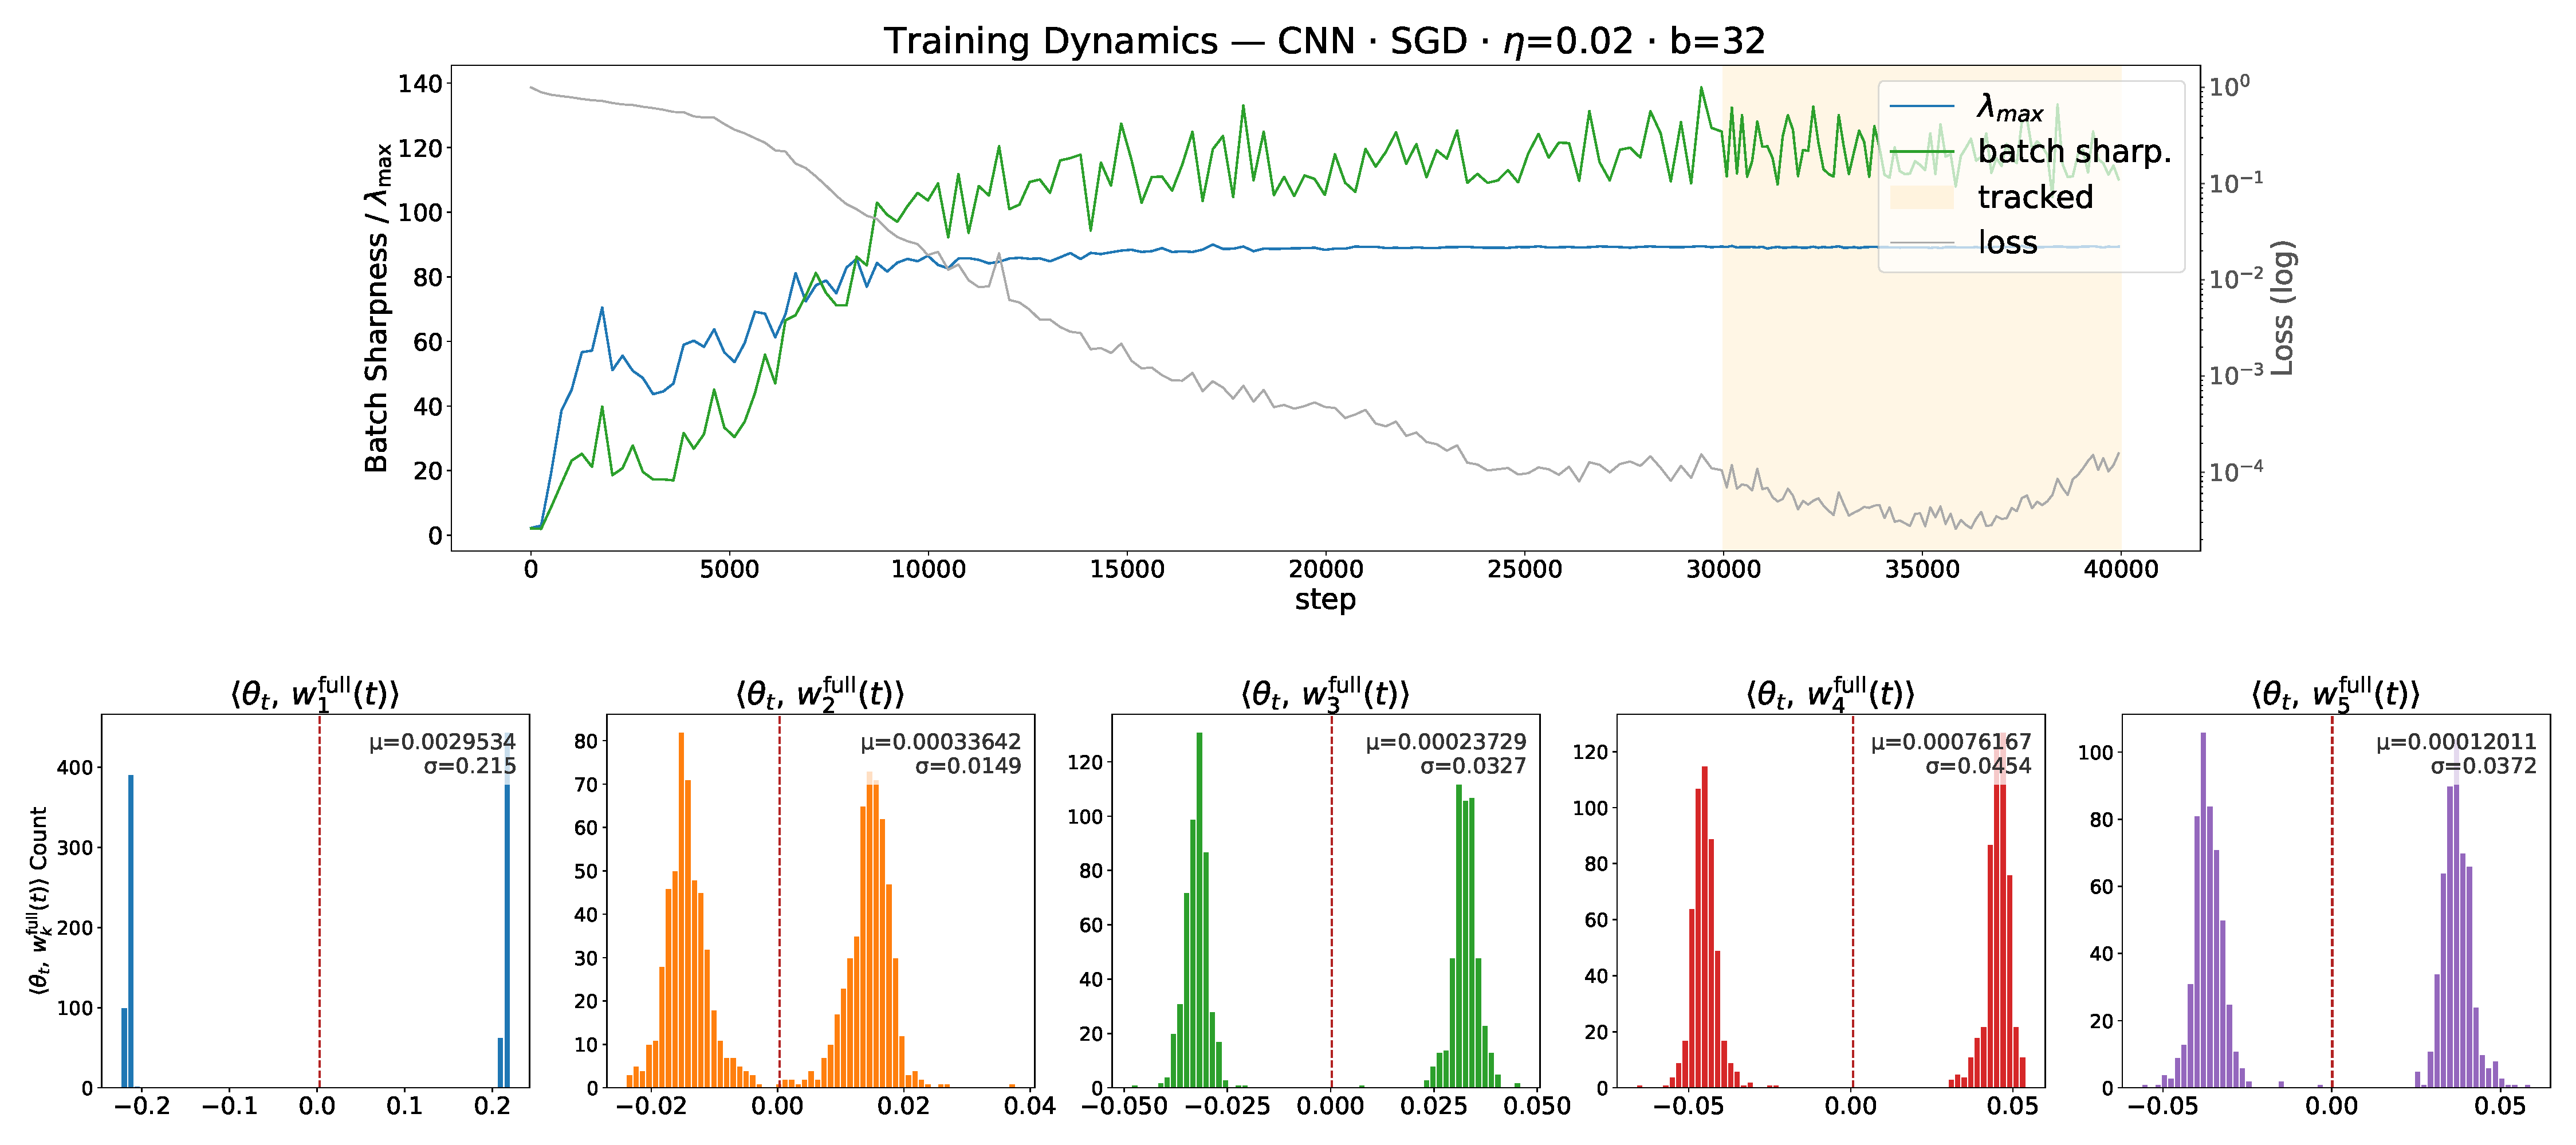
\includegraphics[width=\textwidth]{img/CNN_SGD_lr0.02_b32.pdf}

    \vspace{0.5em}

    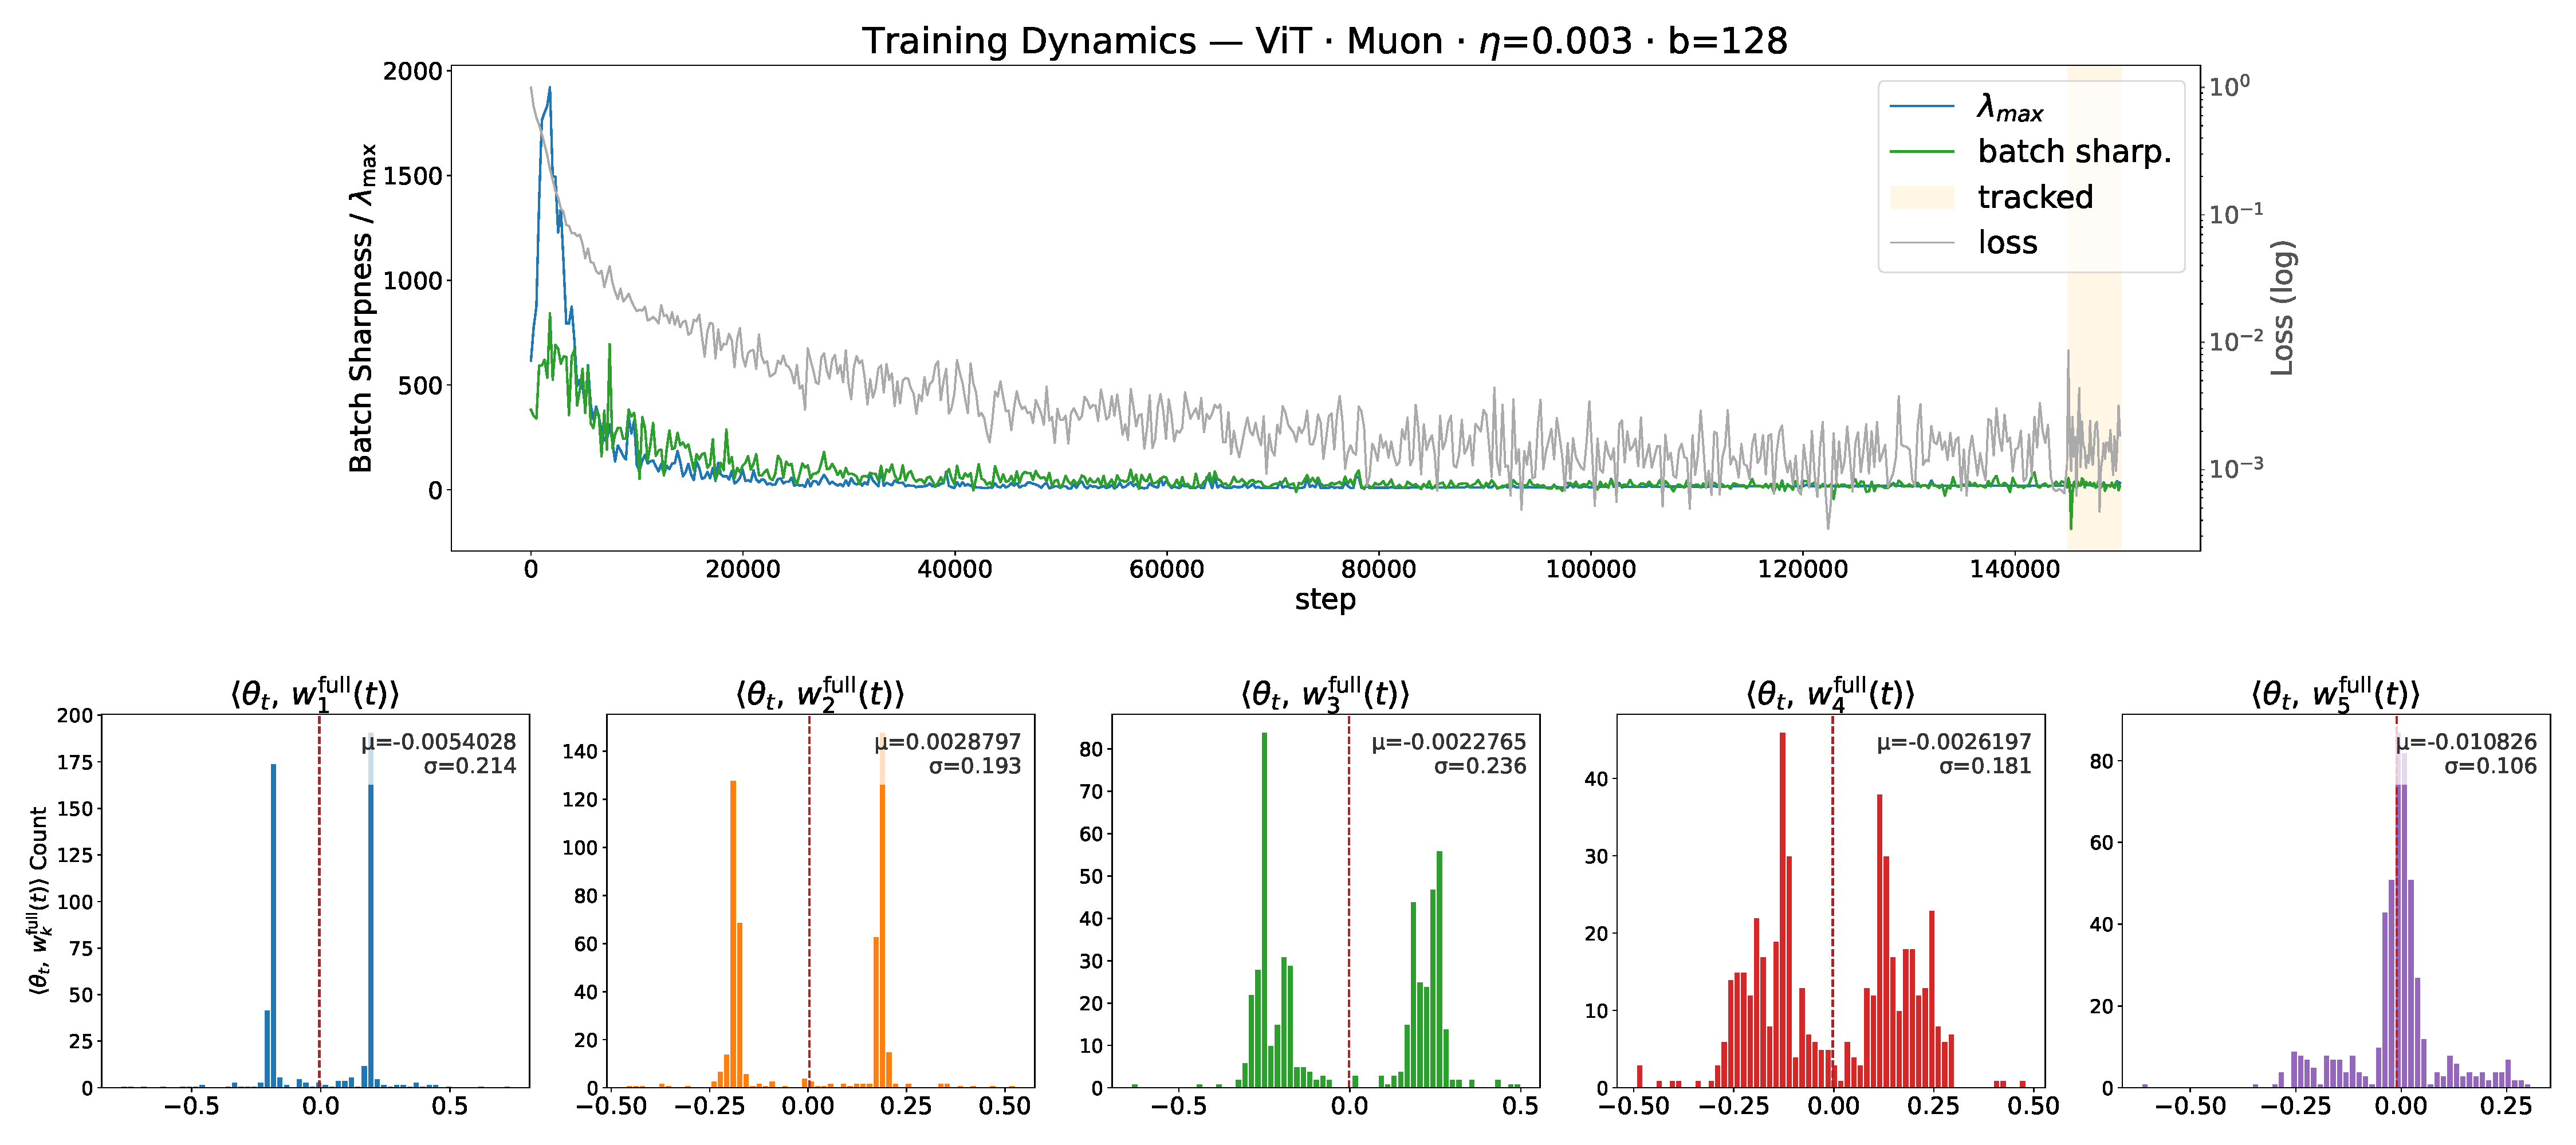
\includegraphics[width=\textwidth]{img/ViT_Muon_lr0.003_b128.pdf}

    \vspace{0.5em}

    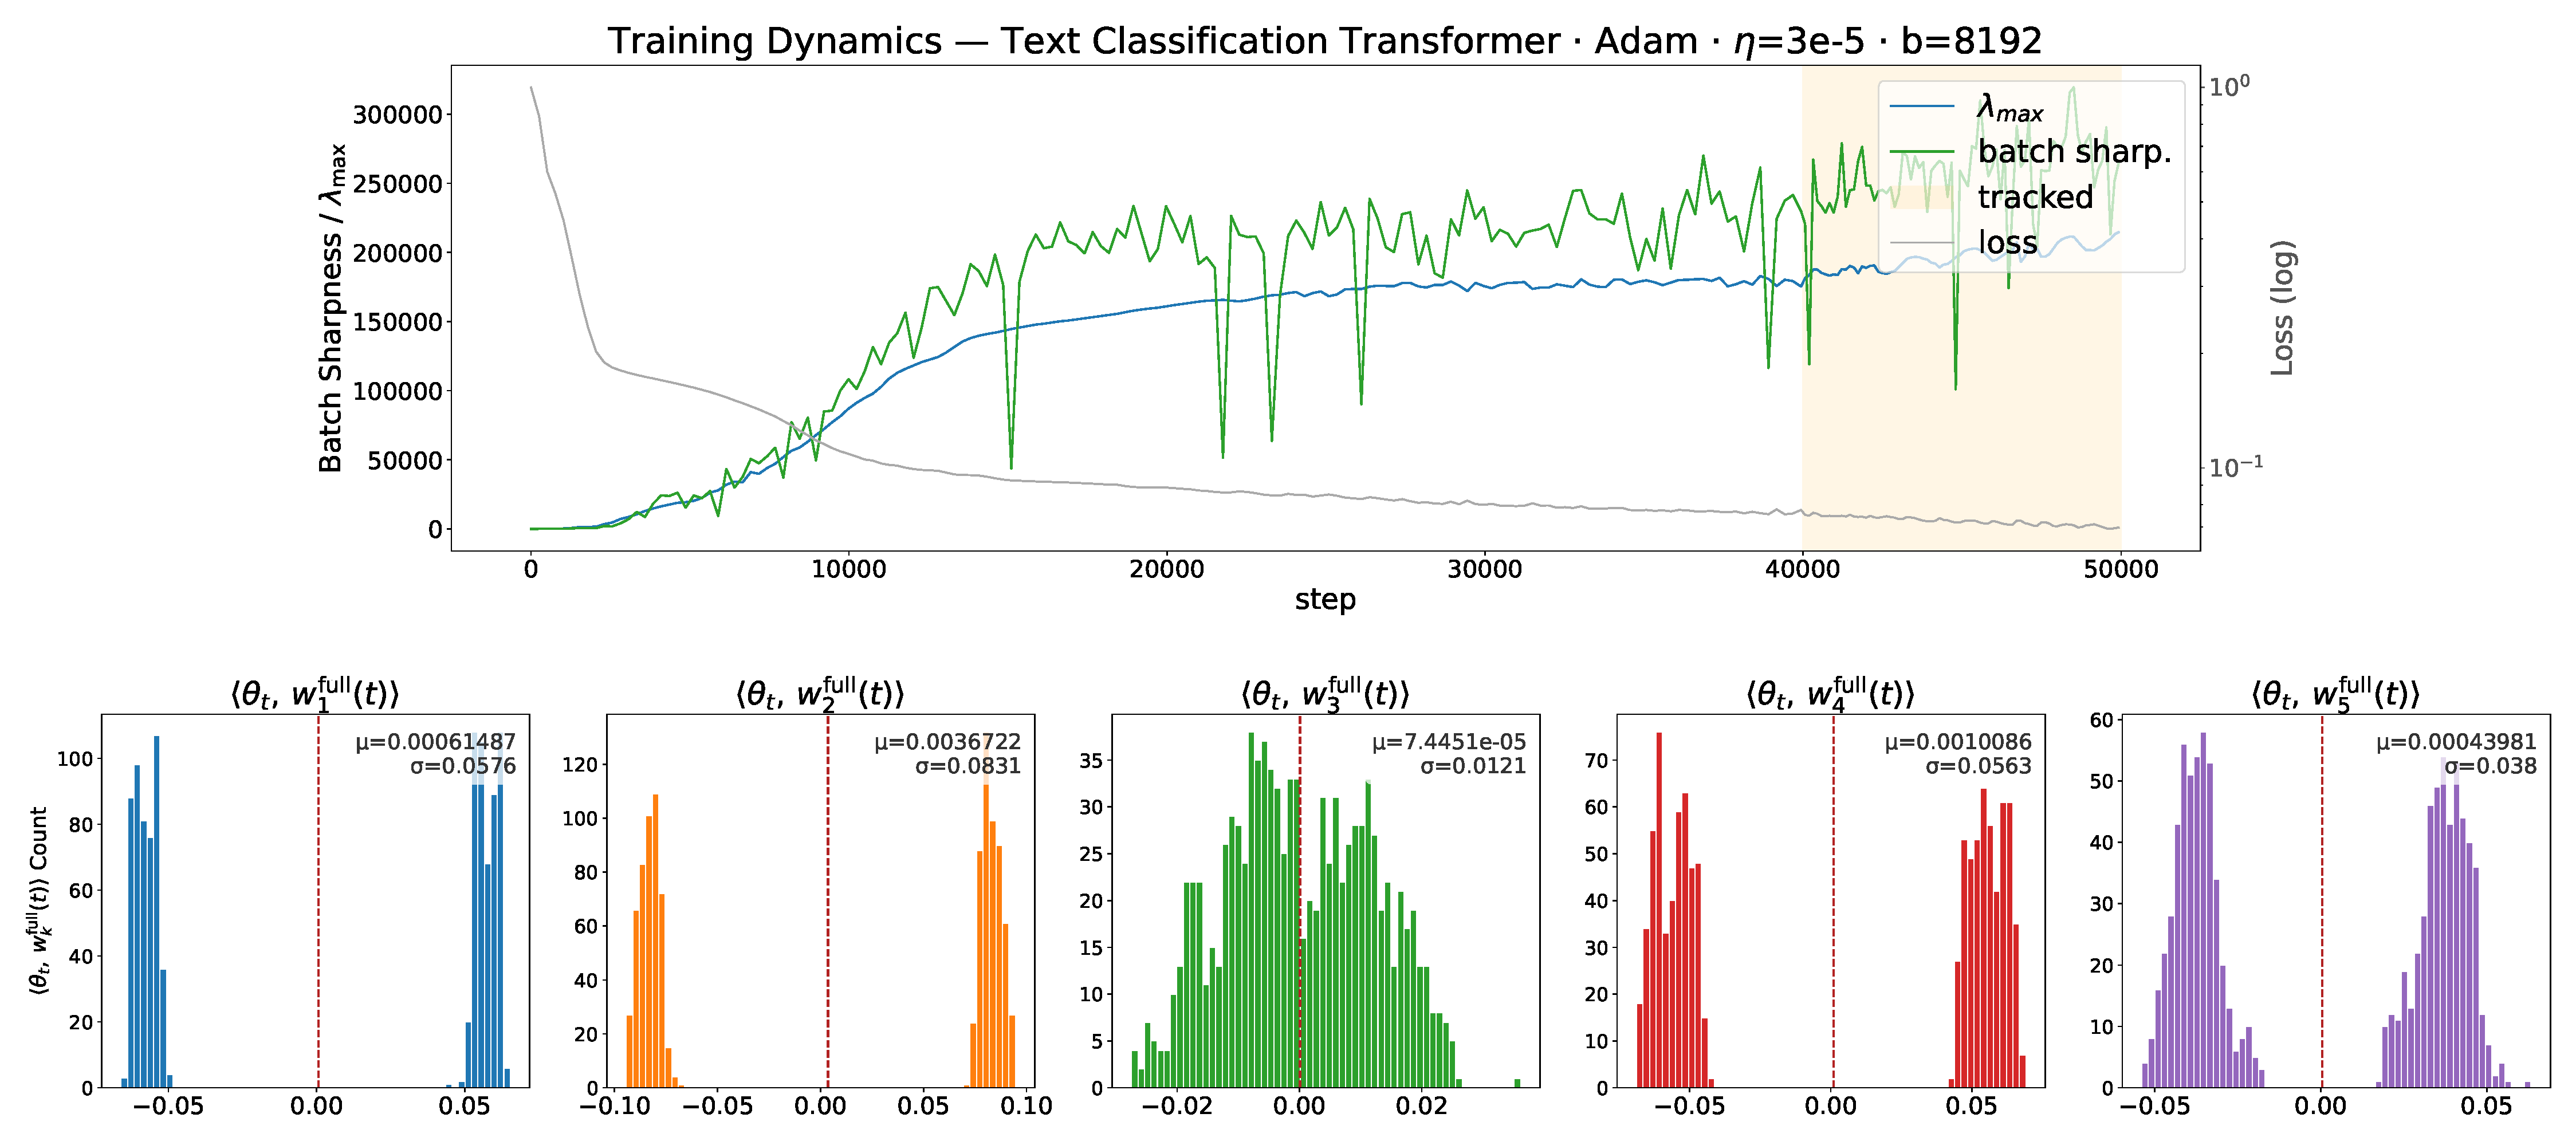
\includegraphics[width=\textwidth]{img/SST_Adam_lr3e-05_b8192.pdf}

    \caption{Bimodal oscillations at the Edge of Stochastic Stability across architectures. Top: training dynamics showing batch sharpness and $\lambda_{\max}$ converging towards the EoSS plateau. Bottom: histograms of $\langle \theta_t, w_k^{\mathrm{full}}(t) \rangle$, the projection of the iterate onto the top-$k$ full-batch Hessian eigenvectors, which is collected within the tracking window shaded in yellow. The characteristic two-peak distribution along leading eigenvectors indicates that the parameter vector oscillates between two modes at each gradient step, a phenomenon we observe consistently across architectures, optimizers, and hyperparameters. This figure exemplifies this with a CNN and Vision Transformer on the Cifar10 classification task, and a Text Classifier Transformer on the SST-2 task.}
    \label{fig:bimodal_eoss_across_architectures}
\end{figure}


% \begin{assumption}\label{ass:global}
% In addition to the local hypotheses of Theorem~\ref{thm:A} (namely $f\in C^5$
% near $\xbar$, $f'(\xbar)=0$, $a=f''(\xbar)>0$, and $D=3b^2-ac>0$), assume:
% \begin{enumerate}[label=\textup{(A\arabic*)}]
% \item \textup{(Confinement.)} $f\in C^2(\R)$ and there exist $R_0>0$, $c_f>0$
% such that $x\,f'(x)\ge c_f\,x^{2}$ for all $|x|\ge R_0$; equivalently the
% gradient points inward outside a compact set. 
% \item \textup{(Step-size admissibility.)} The step size satisfies
% $\eta<2/\sup_{|x|\ge R_0}f''(x)$ on the confinement region, so that
% $F_\eta$ is a contraction toward the origin outside $[-R_0,R_0]$:
% there are $\kappa\in(0,1)$, $b_F<\infty$ with $|F_\eta(x)|\le\kappa|x|+b_F$.
% \item \textup{(Noise tail.)} The i.i.d.\ innovations $\xi_t$ are mean zero,
% unit variance, and sub-Gaussian: $\E[e^{s\xi_t}]\le e^{s^2 K^2/2}$ for all
% $s\in\R$ and some $K<\infty$.
% \end{enumerate}
% \end{assumption}

% \begin{definition}[Local lobe data]\label{def:lobe}
% Fix the $+$ lobe $p_+$ from Theorem~\ref{thm:A} and write $\delta_t:=r_t-p_+$.
% Define
% \begin{enumerate}[label=\textup{(B\arabic*)},leftmargin=2.2em]
% \item \textup{(multiplier)} $\lambda:=1-\eta f''(p_+)$, with $|\lambda|<1$
% (stability, Theorem~\ref{thm:A});
% \item \textup{(cubic coefficient)} $A:=\tfrac{\eta}{2}f'''(p_+)$;
% \item \textup{(separation)} $\rho:=|p_+-\xbar|=\Theta(\sqrt\tau)$
% (amplitude, Theorem~\ref{thm:A});
% \item \textup{(width)} $w:=\sigma/\sqrt{1-\lambda^{2}}$, the standard deviation of
% the lobe \textup{(}the variance in \eqref{eq:Bmoments}\textup{)}.
% \end{enumerate}
% The bimodality criterion is the single inequality
% \textbf{separation $>$ width}, i.e.\ $\rho>w$, equivalently a cap on the noise
% variance, $\sigma^{2}<(1-\lambda^{2})\rho^{2}$.
% \end{definition}
\begin{theorem}
Under the standing assumptions, $\tau \le \tau_0$, and $\sigma \le \sigma_c$
(Eq.~(15)), the quasi-stationary law of the displacement $\delta = X - p_+$ on
the $+$ lobe satisfies
\[
  \mathbb{E}[\delta]
    = \Bigl[\frac{(\lambda_- B_+ + \lambda_+^2 B_-)(1+\lambda_-^2)}{1-\mu^2}
      + B_-\Bigr]\frac{\sigma^2}{1-\mu} + O(\sigma^3),
\]
\[
  \mathrm{Var}(\delta)
    = \frac{(1+\lambda_-^2)\,\sigma^2}{1-\mu^2} + O(\sigma^4),
\]
with $\mu = \lambda_+\lambda_-$ and $B_\pm = -\tfrac{\eta}{2}f'''(p_\pm)$. .
\end{theorem}
% \begin{theorem}[Metastable two-lobe law]
% Under the standing assumptions, let $\sigma \le \sigma_c$ and $\tau \le \tau_0$.
% Started within $O(w)$ of $p_+$ at an even step, the following hold on every time
% horizon $T \ll e^{\,c_0\rho^2/w^2}$:

% \smallskip
% \noindent\textup{(i)} \textbf{Metastable confinement.}\;
% With probability at least $1 - CT\,e^{-c_0\rho^2/w^2}$, the even iterates remain in
% $[p_+-r_0,\,p_++r_0]$ and the odd iterates in $[p_--r_0,\,p_-+r_0]$
% (Lemma~3). The relevant object is therefore the quasi-stationary law of the
% iterates conditioned on non-exit.

% \smallskip
% \noindent\textup{(ii)} \textbf{Per-lobe shape.}\;
% By the truncation transfer (Theorem~\ref{thm:truncation}), the quasi-stationary
% law of $\delta = X - p_+$ on the $+$ lobe has, as $\sigma \to 0$,
% \[
%   \mathbb{E}[\delta]
%     = \Bigl[\tfrac{(\lambda_- B_+ + \lambda_+^2 B_-)(1+\lambda_-^2)}{1-\mu^2}
%       + B_-\Bigr]\frac{\sigma^2}{1-\mu} + O(\sigma^3),
%   \qquad
%   \mathrm{Var}(\delta) = \frac{(1+\lambda_-^2)\sigma^2}{1-\mu^2} + O(\sigma^4),
% \]
% and $\gamma_1(\delta) = O(\sigma) \to 0$, so each lobe is Gaussian to leading
% order. The $-$ lobe law is obtained by exchanging $+ \leftrightarrow -$.

% \smallskip
% \noindent\textup{(iii)} \textbf{Modality.}\;
% The time-averaged law of the iterates is the balanced mixture
% $\tfrac12(\text{$+$ lobe}) + \tfrac12(\text{$-$ lobe})$, the equal weights
% following from strict alternation between lobes. This mixture is bimodal iff the
% separation exceeds the width,
% \[
%   \rho \;>\; \sqrt{\mathrm{Var}(\delta)}.
% \]
% \end{theorem}




% \begin{theorem}[Shape of the lobe and bimodality]\label{thm:B}
% Under Assumption~\ref{ass:global} and Definition~\ref{def:lobe}, for $\sigma$
% small the stationary law of $\delta=r-p_+$ near the $+$ lobe satisfies
% \begin{equation}\label{eq:Bmoments}
%   \E[\delta]
%             =\frac{f'''(p_+)\,\sigma^{2}}{2f''(p_+)\,\bigl(2-\eta f''(p_+)\bigr)^{2}}+O(\sigma^{4}),
%   \quad
%   \Var(\delta)=\frac{\sigma^{2}}{1-\lambda^{2}}+O(\sigma^{4}),
% \end{equation}
% \begin{equation}\label{eq:Bmoments2}
%   \text{skewness}\ \ \gamma_1:=\frac{\mu_3}{\Var(\delta)^{3/2}}=O(\sigma)\xrightarrow{\sigma\to0}0,
%   \qquad
%   \text{excess kurtosis}\ \ \gamma_2:=\frac{\mu_4}{\Var(\delta)^{2}}-3=O(\sigma^{2})\xrightarrow{\sigma\to0}0,
% \end{equation}
% where $\mu_3,\mu_4$ are the third and fourth central moments of $\delta$. Both
% normalised shape measures vanish as $\sigma\to0$, so the lobe is Gaussian to
% leading order, centred at $p_++\E[\delta]$ with width $w$, and the
% mean drift obeys $\sgn(\E\delta)=\sgn(f'''(p_+))$. Consequently the full iterate
% law is a balanced pair of such Gaussians at $\pm(p_++\E\delta)$, which is
% \emph{bimodal} iff $\rho>w$. Using the explicit values
% $1-\lambda^{2}=4a\tau+O(\tau^{2})$ and $\rho^{2}=\dfrac{3a^{3}}{D}\tau+O(\tau^{2})$
% from Theorem~\ref{thm:A}, this reads
% \begin{equation}\label{eq:Bbimodal}
%   \sigma^{2}\;<\;(1-\lambda^{2})\,\rho^{2}\;=\;\frac{12\,a^{4}}{D}\,\tau^{2}\,(1+O(\sqrt\tau))
%   \qquad\Longleftrightarrow\qquad
%   \sigma\;<\;\frac{2a^{2}\sqrt{3}}{\sqrt{D}}\,\tau\,(1+O(\sqrt\tau)),
% \end{equation}
% and unimodal when the reverse strict inequality holds.
% \end{theorem}



%  Translate so the minimum is at $\xbar=0$;
% $a=f''(0)>0$, $b=f'''(0)$, $c=f''''(0)$, $D=3b^2-ac>0$, $\eta=\eta_0+\tau$ with
% $\eta_0=2/a$, and $F_\eta(x)=x-\eta f'(x)$. Theorem~A gives the stable $2$-cycle
% $\{\pp,\pmm\}$ with
% \begin{equation}
% \rho^2=\frac{3a^3}{D}\,\tau+O(\tau^2),\qquad
% \tfrac12(\pp+\pmm)=-\frac{3a^2b}{2D}\,\tau+O(\tau^2),\qquad
% (F_\eta^2)'(\pp)=1-4a\tau+O(\tau^2).
% \label{eq:thmA}
% \end{equation}
% All three were re-derived symbolically and confirmed numerically; they are
% unchanged.
 


% \paragraph{Local expansions at both lobes.} Since $F_\eta\in C^3$, Taylor's theorem at
% each orbit point gives, for small displacements $d,e$,
% \begin{align}
% F_\eta(\pp+d)&=\pmm+\lambda_+\,d+B_+\,d^2+O(d^3),
% \label{eq:Fp}\\
% F_\eta(\pmm+e)&=\pp+\lambda_-\,e+B_-\,e^2+O(e^3),
% \label{eq:Fm}
% \end{align}
% where, using $F_\eta'(r)=1-\eta f''(r)$ and $F_\eta''(r)=-\eta f'''(r)$,
% \[
% \lambda_\pm:=F_\eta'(p_\pm)=1-\eta f''(p_\pm),\qquad
% B_\pm:=\tfrac12 F_\eta''(p_\pm)=-\tfrac\eta2 f'''(p_\pm).
% \]
% The constant terms are fixed by the orbit relations $F_\eta(\pp)=\pmm$,
% $F_\eta(\pmm)=\pp$. The orbit is a fixed point of $G$ with multiplier
% $G'(\pp)=F_\eta'(\pmm)F_\eta'(\pp)=\lambda_-\lambda_+=:\mu$; stability is $|\mu|<1$, a
% condition on the \emph{product}, so the individual $|\lambda_\pm|$ need not be below one.
 

 
% \paragraph{Substitution.} Insert \eqref{eq:eps} into \eqref{eq:dprime}. The
% linear-in-$\varepsilon$ part is
% \[
% \lambda_-\varepsilon_t=\underbrace{\lambda_+\lambda_-}_{\mu}\delta_t
% +\lambda_-B_+\,\delta_t^2+\lambda_-\sigma\xi_t,
% \]
% and, squaring \eqref{eq:eps} and keeping terms of total order $\le2$ in $(\delta_t,\sigma)$,
% \[
% \varepsilon_t^2=\lambda_+^2\delta_t^2+2\lambda_+\sigma\,\delta_t\xi_t+\sigma^2\xi_t^2
% +O(\text{order}\ge3),
% \qquad
% B_-\varepsilon_t^2=\lambda_+^2B_-\,\delta_t^2+2\lambda_+B_-\,\sigma\delta_t\xi_t
% +B_-\,\sigma^2\xi_t^2+O(\ge3).
% \]
% Adding $\lambda_-\varepsilon_t$, $B_-\varepsilon_t^2$, and the fresh kick
% $\sigma\xi_{t+1}$ gives the recursion.
 
% \begin{lemma}[Two-step return recursion]\label{lem:rec}
% With $\mu=\lambda_+\lambda_-$ and $B_\pm=-\tfrac\eta2 f'''(p_\pm)$,
% \begin{equation}
% \delta_{t+2}=\underbrace{\mu\,\delta_t}_{\text{contraction}}
% +\underbrace{\lambda_-\sigma\xi_t+\sigma\xi_{t+1}}_{\text{two kicks per cycle}}
% +\underbrace{\big(\lambda_-B_++\lambda_+^2B_-\big)\delta_t^2
% +2\lambda_+B_-\,\sigma\delta_t\xi_t+B_-\,\sigma^2\xi_t^2}_{\text{quadratic}}
% +O(\sigma^3,\delta_t^3).
% \label{eq:recursion}
% \end{equation}
% Each coefficient was verified by exact symbolic computation; the dropped terms
% ($B_+^2B_-\delta^4$, $2\lambda_+B_+B_-\delta^3$, $2B_+B_-\sigma\delta^2\xi_t$) are all of
% total order $\ge3$.
% \end{lemma}
 
% This is the corrected version of the roadmap's two-step recursion. The key change is
% that the two substeps carry \emph{different} multipliers $\lambda_+,\lambda_-$, where the
% draft used a single $\lambda$. Three features matter downstream: (i) the surviving
% propagated kick is $\lambda_-\sigma\xi_t$ (not $\lambda\sigma\xi_t$) --- the Step-1 kick
% acquires the slope $\lambda_-$ of the lobe it passes through --- so the total linear noise
% has variance $(1+\lambda_-^2)\sigma^2$; (ii) the $\delta_t^2$ coefficient is exactly the
% half-curvature of the two-step map, $\tfrac12 G''(\pp)=\lambda_-B_++\lambda_+^2B_-$
% (directly: $G''=(F_\eta''\!\circ F_\eta)(F_\eta')^2+(F_\eta'\!\circ F_\eta)F_\eta''$,
% giving $2B_-\lambda_+^2+2\lambda_-B_+$ at $\pp$); (iii) the term $B_-\sigma^2\xi_t^2$ is the
% only one with nonzero stationary mean ($\E\xi_t^2=1$), and is the seed of the
% $O(\sigma^2)$ drift, carrying $B_-$ --- the curvature at the \emph{intermediate} lobe.
 
% Assume the innovations $\xi_t$ are i.i.d., mean zero, unit variance, symmetric, with
% $\E\xi^4=\kappa+3$.
 

 
% \begin{proof}
% \emph{Variance.} The linear part of \eqref{eq:recursion} is
% $\delta^{(1)}_{t+2}=\mu\,\delta^{(1)}_t+\lambda_-\sigma\xi_t+\sigma\xi_{t+1}$. The two
% fresh kicks are independent of $\delta^{(1)}_t$ and of each other, with total kick
% variance $(\lambda_-^2+1)\sigma^2$. The stationary second moment obeys
% $M_2=\mu^2 M_2+(\lambda_-^2+1)\sigma^2$, giving
% $M_2=(1+\lambda_-^2)\sigma^2/(1-\mu^2)$. Since $\E\delta=O(\sigma^2)$ (below),
% $\Var(\delta)=M_2+O(\sigma^4)$, which is \eqref{eq:var}.
 
% \emph{Drift.} Take the stationary expectation of \eqref{eq:recursion}. The fresh-noise
% terms and the cross term $2\lambda_+B_-\sigma\,\E[\delta_t\xi_t]=0$ vanish; only
% $B_-\sigma^2\,\E[\xi_t^2]=B_-\sigma^2$ survives among the noise terms. With
% $\Delta:=\E\delta$,
% \[
% \Delta=\mu\Delta+(\lambda_-B_++\lambda_+^2B_-)\,M_2+B_-\sigma^2+O(\sigma^4),
% \]
% so $(1-\mu)\Delta=(\lambda_-B_++\lambda_+^2B_-)M_2+B_-\sigma^2$. Substituting
% $M_2=(1+\lambda_-^2)\sigma^2/(1-\mu^2)$ gives \eqref{eq:drift} and confirms
% $\Delta=O(\sigma^2)$.
 
% \emph{Skewness.} Expand $\delta=\Delta+u^{(1)}+u^{(2)}+\cdots$ with $u^{(1)}=O(\sigma)$
% the centred linear part (Gaussian, $\E[(u^{(1)})^3]=0$) and $u^{(2)}=O(\sigma^2)$ the
% quadratic part. With symmetric noise the leading third central moment is
% $\mu_3=3\,\E[(u^{(1)})^2(u^{(2)}-\E u^{(2)})]+O(\sigma^6)=O(\sigma^4)$, since each
% factor contributes its own power of $\sigma$. Because $\Var(\delta)=\Theta(\sigma^2)$,
% the normalised skew is $\gamma_1=\mu_3/\Var^{3/2}=O(\sigma)\to0$. The lobe is therefore
% Gaussian to leading order, the cubic landscape term entering only at next order.
% \end{proof}
 
% \begin{remark}[What is unchanged from the draft]
% The structural conclusion of the original Theorem~4 --- each lobe Gaussian to leading
% order, drift at $O(\sigma^2)$, normalised skew $O(\sigma)\to0$ --- is correct and
% survives verbatim; it does not depend on the multiplier bookkeeping. Only the exact
% constants in \eqref{eq:var}--\eqref{eq:drift} (and the $\mu_3$ coefficient, eq.~(19)
% of the draft) change.
% \end{remark}
 
% \section{Leading order in \texorpdfstring{$\tau$}{tau}, and the surviving threshold}
 
% As $\tau\to0$, $\lambda_-\to-1$, $\mu\to1$, $1-\mu^2=(1-\mu)(1+\mu)\to 8a\tau$, so
% \begin{equation}
% \Var(\delta)=\frac{(1+\lambda_-^2)\sigma^2}{1-\mu^2}
% \;\longrightarrow\;\frac{2\sigma^2}{8a\tau}=\frac{\sigma^2}{4a\tau}.
% \label{eq:varlead}
% \end{equation}
% This is exactly the leading-order width the draft reported (via the mislabelled
% $1-\lambda^2=4a\tau$). Combined with $\rho^2=3a^3\tau/D$ from \eqref{eq:thmA}, the
% bimodality criterion $\rho>\sqrt{\Var(\delta)}$ reads
% \begin{equation}
% \frac{3a^3\tau}{D}>\frac{\sigma^2}{4a\tau}
% \;\Longleftrightarrow\;
% \sigma^2<\frac{12a^4}{D}\,\tau^2
% \;\Longleftrightarrow\;
% \sigma<\frac{2a^2}{\sqrt3\,\sqrt D}\,\tau\,(1+o(1)),
% \label{eq:threshold}
% \end{equation}


% The drift \eqref{eq:drift} scales as $\Delta\sim\,$const$\cdot\tau^{-3/2}\sigma^2$ and is
% \emph{negative} (directed toward the origin) in every landscape tested; see
% Section~\ref{sec:num}. In particular the draft's claim $\sgn(\E\delta)=\sgn f'''(\pp)$
% is false. The drift's sign is set by the full combination
% $\lambda_-B_++\lambda_+^2B_-$ together with the $B_-$ term, not by $f'''(\pp)$ alone,
% and the prediction ``$E[r^2]$ shift flips with $\sgn U'''(a)$'' (Prediction~2 of the
% draft) should be withdrawn or restated; the robust, testable statement is that the
% mean-square radius is \emph{suppressed} (the iterate drifts toward $0$) by $O(\sigma^2)$.

% \subsection{Generalized predictor dynamics for SGD}
 
% With phase-corrected amplitude $m_t=\E[r_t]$, mean sharpness deviation
% $\bar y_t$, lobe variance $V_t$, gradient-noise variance along the top
% eigenvector $\sigma_u^2=\bm u^\top\bm\Sigma_b\bm u$ (which scales as $1/b$ in
% the batch size $b$), and $q_t=\E[r_t^2]=m_t^2+V_t$:
% \begin{align}
%   m_{t+1}&=(1+\eta\bar y_t)\,m_t+\eta F'(m_t)+\tfrac{\eta}{2}F'''(m_t)\,V_t+O(V_t^2),
%   \label{eq:mfm}\\[2pt]
%   \bar y_{t+1}&=\bar y_t+\eta\Bigl(\alpha-\tfrac{\beta}{2}\,\underbrace{(m_t^2+V_t)}_{=\,q_t}\Bigr)
%   \;=\;\bar y_t+\tfrac{\eta\beta}{2}\bigl(\rho_\star^2-m_t^2-V_t\bigr),
%   \label{eq:mfy}\\[2pt]
%   V_{t+1}&=\bigl(1+\eta\bar y_t+\eta F''(m_t)\bigr)^{2}V_t+\eta^2\sigma_u^2+O(V_t^2,\sigma_u^4).
%   \label{eq:mfV}
% \end{align}

\section{Generalized predictor dynamics for noise-injected GD}


In the Hessian eigenbasis at a reference point near a minimum, let $z$ denote the
\emph{normal} (sharp) coordinate, oscillating at the edge of stability, and let
$y_i$, $i\ge 2$, denote the \emph{tangent} coordinates. The loss is
\begin{equation}
L \;=\; \frac{\lambda_z}{2}z^2 + \frac{c_4}{24}z^4 
\;+\; \sum_{i\ge 2}\Big( \frac{\lambda_i}{2}y_i^2 + \beta_i\, z^2 y_i \Big),
\qquad \eta\lambda_z > 2,\;\; \eta\lambda_i < 2.
\label{eq:loss}
\end{equation}
The gradient components are
\begin{align}
\partial_z L &= \Big(\lambda_z + 2\textstyle\sum_i \beta_i y_i\Big) z
 + \frac{c_4}{6}z^3, \label{eq:dzL}\\
\partial_{y_i} L &= \lambda_i y_i + \beta_i z^2. \label{eq:dyL}
\end{align}
The stochastic gradient-descent recursion with step size $\eta$ and injected noise is
\begin{align}
z_{t+1} &= z - \eta\,\partial_z L + \sigma_z\xi, \label{eq:zupdate}\\
y_{i+1} &= y_i - \eta\,\partial_{y_i}L + \sigma_i\xi_i, \label{eq:yupdate}
\end{align}
with $\xi,\xi_i$ i.i.d., mean zero, unit variance, mutually independent, and independent
of the current state. Throughout, $C^5$ smoothness and a sub-Gaussian noise tail are
assumed so that all moments below exist.


\paragraph{Notations.} Because $z$ flips sign each step at the edge, we factor out the
oscillation by writing
\begin{equation}
z_t = (-1)^t\,(\nu_t + \delta_t),\qquad \E[\delta_t]=0,\qquad V_t := \Var(\delta_t).
\label{eq:lobeframe}
\end{equation}
Here $\nu_t$ is the (signed) lobe center and $\delta_t$ the within-lobe fluctuation.
We also split each tangent coordinate into mean and fluctuation,
\begin{equation}
y_{i,t} = \ybar_{i,t} + \ytil_{i,t},\qquad \E[\ytil_{i,t}]=0,\qquad
V_{y_i,t} := \Var(y_{i,t}) = \E[\ytil_{i,t}^2].
\label{eq:ysplit}
\end{equation}
Finally we define the \emph{sharpness gap}
\begin{equation}
s_t \;:=\; \lambda_z + 2\sum_i \beta_i \ybar_{i,t} - \frac{2}{\eta}.
\label{eq:sdef}
\end{equation}

\section{The joint predictor system}
 
% For easy reference, the four coupled update equations that constitute the full predictor are
% collected here together. They are the object that is analysed in \S\S3--5 above, and whose
% fixed point is solved in \S\ref{sec:fixedpoint} below. 
 
\begin{equation*}
\boxed{\begin{aligned}
\nu_{t+1} &= (1+\eta s_t)\,\nu_t
 + \eta\frac{c_4}{6}\big(\nu_t^3 + 3\nu_t V_t\big)
 &&\textup{(22)}\\[6pt]
V_{t+1} &= \Big(1+\eta s_t + \eta\frac{c_4}{2}\nu_t^2
            \Big)^{\!2} V_t
 + \sigma_z^2
 + 4\eta^2\!\sum_i \beta_i^2\big(\nu_t^2 + V_t\big)V_{y_i,t}
 &&\textup{(23)}\\[6pt]
\ybar_{i,t+1} &= (1-\eta\lambda_i)\,\ybar_{i,t}
 - \eta\beta_i\big(\nu_t^2 + V_t\big)
 &&\textup{(24a)}\\[6pt]
V_{y_i,t+1} &= (1-\eta\lambda_i)^2\,V_{y_i,t} + \sigma_i^2
 &&\textup{(24b)}
\end{aligned}}
\label{eq:predictor}
\end{equation*}
 
\noindent The four unknowns are $(\nu_t, V_t, \ybar_{i,t}, V_{y_i,t})$:
the lobe separation $\nu_t$ (mean of the positive lobe), the within-lobe variance $V_t$,
the tangent means $\ybar_{i,t}$, and the tangent variances $V_{y_i,t}$.
They are coupled through $s_t$ (tangent means enter the normal update via the sharpness gap)
and through $\nu_t^2+V_t=\mathbb E[z_t^2]$ (the oscillation energy, which drives the tangents
in (24a) and supplies the curvature-noise term in (23)).


\section{The fixed point}
\label{sec:fixedpoint}
 
Solving the fixed point for the joint-predictor system we get:
 
\begin{equation*}
\boxed{\begin{aligned}
V_{y_i\star} &= \frac{\sigma_i^2}{\eta\lambda_i(2-\eta\lambda_i)}
&&\text{(tangent noise)}\\[4pt]
\ybar_{i\star} &= -\frac{\beta_i}{\lambda_i}\,(\nu_\star^2+V_\star)
&&\text{(tangent offset $\propto$ oscillation energy)}\\[4pt]
\nu_\star^2\;(\sigma=0) &= \frac{\lambda_{z}-\frac{2}{\eta}}{2\sum \frac{\beta^2_{i}}{\lambda_{i}}-c_4/6}
&&\text{(deterministic oscillation amplitude)}\\[4pt]
V_\star\;(\sigma>0) &= \frac{\sigma_z^2+4\eta^2\rho_\star^2\sum_i\beta_i^2V_{y_i\star}}
{2\eta\frac{|c_4|}{3}\nu_\star^2}
&&\text{(within-lobe width, noise-driven)}
\end{aligned}}
\label{eq:fixedpoint}
\end{equation*}

The tangent-noise and offset are easy to derive since matching the moment condition at stationarity gives the following values. For solving the deterministic oscillation amplitude, we set the variance to be zero and obtain 

\begin{align}
   & \nu = (1+\eta (\lambda_z + 2\sum_i \beta_i \ybar_{i\star}  - \frac{2}{\eta}))\,\nu
 + \eta\frac{c_4}{6}\nu^3 \\
 & \implies 0 = (\lambda_z- \frac{2}{\eta}) -2 \sum_i \frac{\beta_i ^2}{\lambda_{i}} \gamma^2 + \frac{c_4}{6}\nu^2 \\ 
 & \implies \nu_\star^2= \frac{\lambda_{z}-\frac{2}{\eta}}{2\sum \frac{\beta^2_{i}}{\lambda_{i}}-c_4/6}
\end{align}
This condition establishes two things: a) for sub-quartic loss $c_{4}<0$, oscillation exist irrespective of the value of $\beta_{i}$ and b) for super-quartic loss $c_{4}>0$, oscillation can still exist if the third-order joint coupling factor $\beta_{i}$ is large enough so that oscillations are sustained in the joint $(z, y_{i})$ plane.
As we know for a scalar loss super-quartic loss might diverge, but in multi-dimensional setting the cross direction can allow stable oscillation even in the case of super-quartic function.

Similarly, to solve the variance along the largest eigenvector direction only for the case $c_{4}<0$, we have:
\begin{align}
V &= \Big(1+\eta s_\star + \eta\frac{c_4}{2}\nu_\star^2\Big)^{\!2} V
 + \sigma_z^2
 + 4\eta^2\sum_i \beta_i^2\big(\nu_\star^2 + V\big)V_{y_i\star} \\
&\implies V\left[1 - \Big(1+\eta s_\star + \eta\frac{c_4}{2}\nu_\star^2\Big)^{\!2}\right]
= \sigma_z^2 + 4\eta^2\nu_\star^2\sum_i \beta_i^2 V_{y_i\star} \\
&\implies V = \frac{\sigma_z^2 + 4\eta^2\nu_\star^2\sum_i \beta_i^2 V_{y_i\star}}
{1 - \Big(1+\eta s_\star + \eta\frac{c_4}{2}\nu_\star^2\Big)^{\!2}}.
\end{align}
To simplify the denominator, we use the $\nu$-stationarity condition. At the fixed point,
equation~(25) gives $s_\star = -\frac{c_4}{6}\nu_\star^2$, so
\begin{equation}
1 + \eta s_\star + \eta\frac{c_4}{2}\nu_\star^2
= 1 + \eta\nu_\star^2\!\left(-\frac{c_4}{6} + \frac{c_4}{2}\right)
= 1 + \eta\frac{c_4}{3}\nu_\star^2
=: 1 - \eta\frac{|c_4|}{3}\nu_\star^2,
\end{equation}
where the last equality uses $c_4 < 0$. Writing $x := \eta\frac{|c_4|}{3}\nu_\star^2 > 0$,
the denominator becomes
\begin{equation}
1 - (1-x)^2 = 2x - x^2 \approx 2x = 2\eta\frac{|c_4|}{3}\nu_\star^2,
\end{equation}
where we drop $x^2 = O(\Delta^2)$ since $x = O(\Delta)$ is small near the edge of stability.
Substituting back,
\begin{equation}
\boxed{V_\star = \frac{\sigma_z^2 + 4\eta^2\nu_\star^2\sum_i \beta_i^2 V_{y_i\star}}
{2\eta\dfrac{|c_4|}{3}\nu_\star^2}.}
\end{equation}
Note that we can't get a closed-form expression for the case $c_{4}>0$. 
% At $\sigma=0$ the system is exact: $V_\star=0$ and $\nu_\star^2=\Delta/(2B-c_4/6)=:\Delta/\mathcal D$,
% a pure two-point period-2 cycle, with $\mathcal D:=2B-c_4/6$ the orbit-existence discriminant
% (positive whenever the orbit exists). At finite noise, $\nu_\star^2$ and $V_\star$ are solved
% jointly (each equation depends on the other's unknown); the last line is the leading-order
% relation, accurate while $V_\star\ll\nu_\star^2$. Figure~\ref{fig:nuV} confirms this against raw
% SGD: the realized curvature (defined in \S7) tracks the exact formula at all noise levels, while
% $\nu_\star^2$ and $V_\star$ move in opposite directions as $\sigma$ increases (separation shrinks,
% width grows).
 
% Insert \eqref{eq:dzL} into \eqref{eq:zupdate} and collect the multiplier on $z$:
% \begin{equation}
% z' = G\,z + \sigma_z\xi,\qquad
% G := 1 - \eta\Big(\lambda_z + 2\textstyle\sum_i\beta_i y_i\Big)
%  - \eta\frac{c_4}{6}z^2 - \eta\frac{g_6}{120}z^4.
% \label{eq:Gdef}
% \end{equation}
% $G$ is merely a name for ``one minus $\eta$ times the local curvature.'' Substituting the
% lobe frame \eqref{eq:lobeframe} into \eqref{eq:Gdef} and using $z_{t+1}=(-1)^{t+1}(\nu_{t+1}+\delta_{t+1})$,
% divide both sides by $(-1)^{t+1}=-(-1)^t$:
% \begin{equation}
% \nu_{t+1}+\delta_{t+1} = H + (-1)^{t+1}\sigma_z\xi,\qquad H := -G\,(\nu_t+\delta_t),
% \label{eq:Hdef}
% \end{equation}
% where we used that $\pm1$ is its own inverse to keep the noise term's magnitude. Note
% $z^2=(\nu+\delta)^2$ is sign-independent. Expanding $-G$ and splitting $y_i$ via
% \eqref{eq:ysplit},
% \begin{equation}
% -G = \underbrace{\Big[-1+\eta\lambda_z + 2\eta\sum_i\beta_i\ybar_i\Big]}_{\text{const.\ in }\delta,\ytil}
%  + 2\eta\sum_i\beta_i\ytil_i
%  + \eta\frac{c_4}{6}(\nu+\delta)^2 + \eta\frac{g_6}{120}(\nu+\delta)^4.
% \label{eq:negGexpand}
% \end{equation}



% \begin{lemma}[Collapse of the constant block]
% The bracketed constant in \eqref{eq:negGexpand} equals $1+\eta s_t$.
% \end{lemma}
% \begin{proof}
% Multiply \eqref{eq:sdef} by $\eta$: $\eta s_t = \eta\lambda_z + 2\eta\sum_i\beta_i\ybar_i - 2$.
% Add $1$: $1+\eta s_t = \eta\lambda_z + 2\eta\sum_i\beta_i\ybar_i - 1$, which is the bracket
% verbatim. The definition of $s_t$ was \emph{engineered} to absorb the $-2/\eta$ that sits at
% the flip ($\eta\lambda_z = 2 \Leftrightarrow$ multiplier $=-1$).
% \end{proof}
 
% \noindent Therefore, multiplying \eqref{eq:negGexpand} by $(\nu+\delta)$ to form $H=-G(\nu+\delta)$:
% \begin{equation}
% \boxed{\;
% H = (1+\eta s_t)(\nu+\delta)
%  + 2\eta\Big(\sum_i\beta_i\ytil_i\Big)(\nu+\delta)
%  + \eta\frac{c_4}{6}(\nu+\delta)^3
%  + \eta\frac{g_6}{120}(\nu+\delta)^5.
% \;}
% \label{eq:Hfull}
% \end{equation}


% The middle form of \eqref{eq:mfy} is the DNL sharpness feedback
% $\bar y_{t+1}-\bar y_t=\eta(\alpha-\tfrac{\beta}{2}\E[x^2])$ written with
% $\E[x^2]=q_t$; the right form uses \eqref{eq:rhostar}. The \emph{single new term
% relative to GD} is the explicit appearance of $V_t$ in
% \eqref{eq:mfy}: the stabilisation force responds to the full second moment
% $q_t=m_t^2+V_t$, not to $m_t^2$ alone. In full-batch GD, $\sigma_u^2=0$ forces
% $V_t\to0$ and \eqref{eq:mfy} balances at $m^2=\rho_\star^2$, $\bar y=0$,
% i.e.\ sharpness exactly $2/\eta$ (the DNL result). Under SGD, $V$ stays strictly
% positive and the balance shifts.

% \begin{theorem}[Local and global truncation error]
% \label{thm:trunc}
% Let $\{p_+, p_-\}$ be a period-$2$ orbit of the GD map $F(x)=x-\eta\nabla L(x)$,
% and let $\hat\delta^{+}_t$ denote the iterate of the truncated map $(\star)$
% starting from the same initial condition $\hat\delta^{+}_0=\delta^+_0$. Define the
% global error $e_t:=\delta^+_t-\hat\delta^{+}_t$.

% \medskip\noindent
% Assume the following conditions hold.
% \begin{enumerate}[nosep,label=\textup{(\Alph*)}]
% \item \textup{(Contraction)} $|\mu|=|(1-\eta f''(p_+))(1-\eta f''(p_-))|<1$,
% i.e.\ $f''(p_+),f''(p_-)\in(0,2/\eta)$.
% \item \textup{(Loss regularity)} $f\in C^4$ in a neighbourhood of $p_+$ and
% $p_-$, so that
% \[
% A_+ = -\tfrac{\eta}{2}f'''(p_+), \quad
% A_- = -\tfrac{\eta}{2}f'''(p_-), \quad
% B_+ = -\tfrac{\eta}{6}f''''(p_+), \quad
% B_- = -\tfrac{\eta}{6}f''''(p_-),
% \]
% and $P_+ = \lambda_- B_+ + 2\lambda_+ A_+ A_- + \lambda_+^3 B_-$ are all finite,
% where $\lambda_+ = 1-\eta f''(p_+)$ and $\lambda_- = 1-\eta f''(p_-)$.
% \item \textup{(Global confinement)} $L$ satisfies
% $\langle \nabla L(x),\, x-x^\star \rangle \ge c_L \|x-x^\star\|^2$
% for $\|x-x^\star\|\ge R_0$, and $\eta < 2c_L/K^2$ where
% $K=\sup_{\|x-x^\star\|\ge R_0}\|\nabla^2 L(x)\|$,
% ensuring the iterates do not escape to infinity.
% \item \textup{(Noise moments)} $\kappa_2=\mathbb{E}[\xi^2]<\infty$ and
% $\kappa_6=\mathbb{E}[\xi^6]<\infty$.
% \item \textup{(Noise level)} $\sigma^2 < \sigma_c^2 :=
% \dfrac{1-(|\mu|+2|Q_+|\rho_{\max})^2}{4\lambda_+^2 A_-^2 \kappa_2}$,
% where $Q_+ = \lambda_- A_+ + \lambda_+^2 A_-$ and $\rho_{\max}$ is the
% basin radius supplied by condition~\textup{(C)}.
% \end{enumerate}

% \medskip\noindent
% Then the following two statements hold.

% \medskip\noindent
% \textup{(i) Local truncation error.}
% The local error at each step satisfies
% \[
% R_t = P_+(\delta^+_t)^3
% + (2A_+A_- + 3\lambda_+^2 B_-)\,\sigma\,(\delta^+_t)^2\xi_t
% + 3\lambda_+ B_-\,\sigma^2\,\delta^+_t\,\xi_t^2
% + B_-\,\sigma^3\,\xi_t^3
% + O(\text{order }4),
% \]
% and its mean-square size is
% \begin{align*}
% \mathbb{E}[R_t^2]
% &= P_+^2\,\mathbb{E}[(\delta^+_t)^6]
% + (2A_+A_-+3\lambda_+^2 B_-)^2\,\sigma^2\,\mathbb{E}[(\delta^+_t)^4]\,\kappa_2 \\
% &\quad + 9\lambda_+^2 B_-^2\,\sigma^4\,\mathbb{E}[(\delta^+_t)^2]\,\kappa_4
% + B_-^2\,\sigma^6\,\kappa_6
% \;=\; O(\sigma^6).
% \end{align*}
% In particular $\|R_t\|_2 = O(\sigma^3)$:
% \textbf{the truncation is locally third order.}

% \medskip\noindent
% \textup{(ii) Global truncation error.}
% The global error satisfies, uniformly over all $T=2N$,
% \[
% \sup_{N\ge 1}\,\mathbb{E}[e_{2N}^2]
% \;\le\;
% \frac{C\,\sigma^6}{(1-\sqrt{\Lambda})^2}
% \;=\; O(\sigma^6),
% \]
% where
% \[
% \Lambda = (|\mu|+2|Q_+|\rho_{\max})^2 + 4\lambda_+^2 A_-^2 \kappa_2\,\sigma^2 < 1
% \]
% under conditions~\textup{(A)--(E)}, and $C$ depends only on $f$, $\eta$,
% and the moments of $\xi$.
% In particular $\|e_T\|_2 = O(\sigma^3)$ \textbf{uniformly in $T$}: the
% accumulated truncation error stays at third order for all time and does not
% blow up.

% \medskip\noindent
% Consequently the stationary mean $\Delta_+$ and variance $V_+$ of the exact
% chain differ from those of the truncated chain $(\star)$ by $O(\sigma^3)$ and
% $O(\sigma^4)$ respectively, so the boxed formulae \textup{(5$_+$)} and
% \textup{(6)} are correct through $O(\sigma^2)$.
\end{theorem}
\begin{figure}
    \centering
    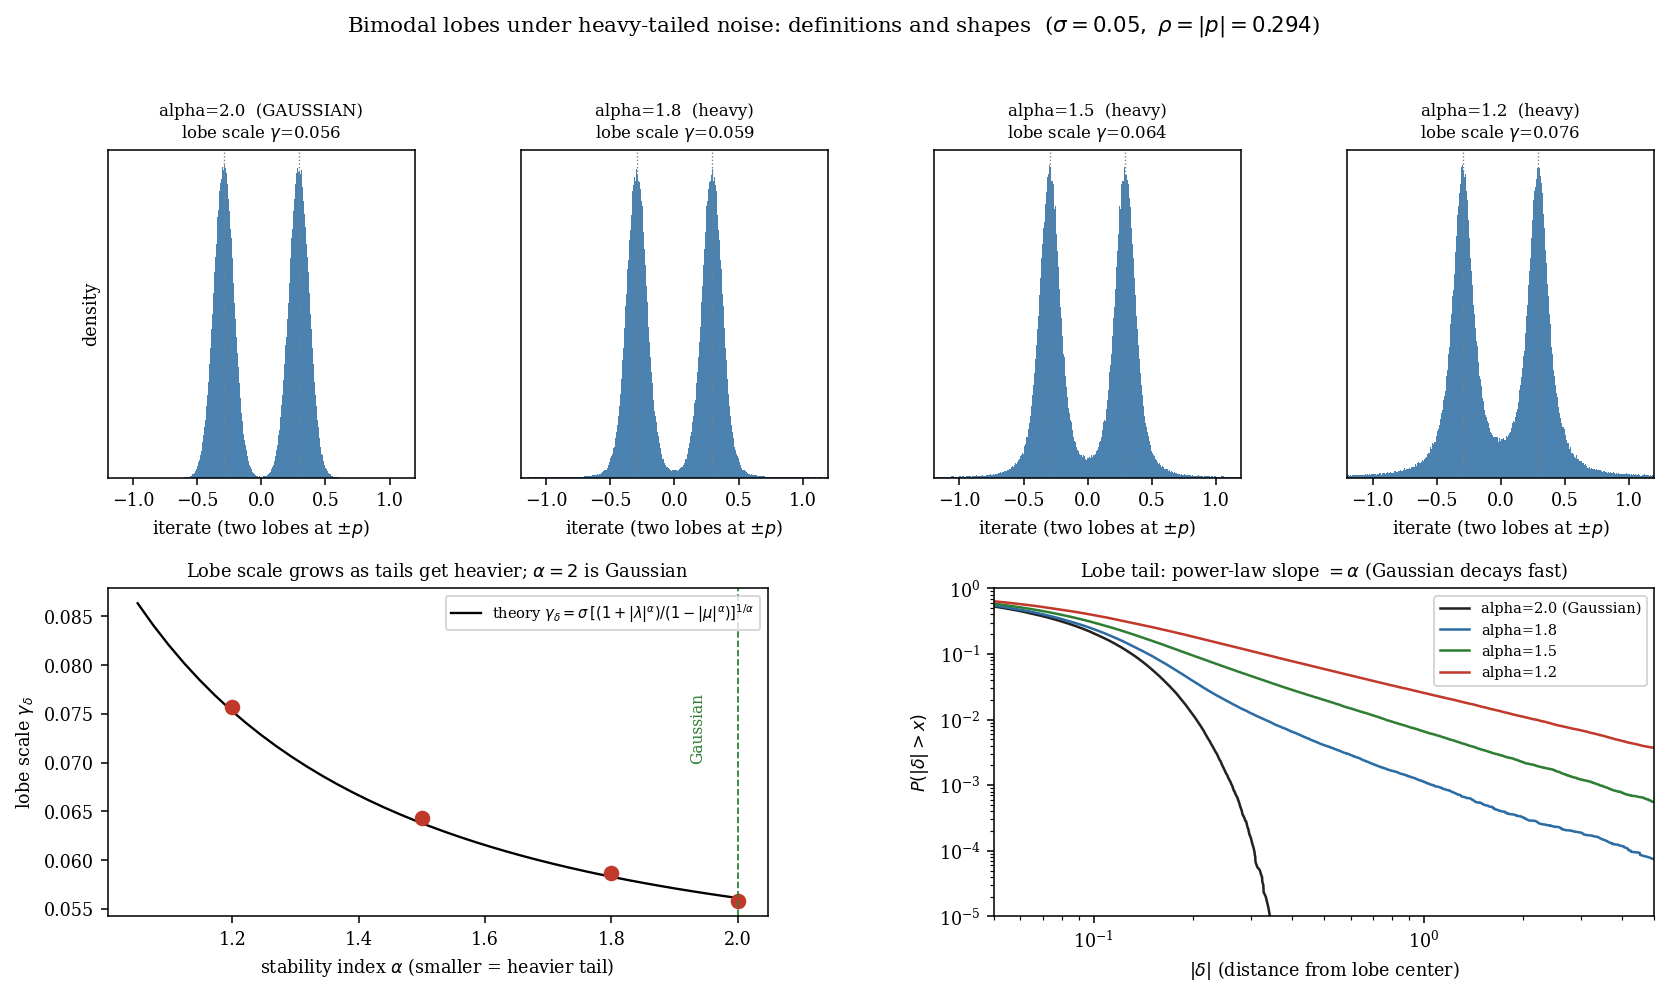
\includegraphics[width=0.9\linewidth]{img/bimodal_heavytail_defined.png}
\end{figure}

\bibliography{iclr2026_conference}
\bibliographystyle{iclr2026_conference}


\appendix
\section{Appendix}
You may include other additional sections here.

\begin{remark}[Finite noise]
For $\sigma>0$ the kernel is strictly positive, so $p(0)>0$ and literal
depletion is smoothed below scale $r_B$; the finite-noise modality
criterion is $p''_{\eta,\sigma}(0)>0$, whose threshold converges to
$\eta_{\mathrm H}$ as $\sigma_{\mathrm{eff}}\to0$.
\end{remark}

\begin{remark}[Continuous curvature]
If the curvature density is positive at $h^\ast=1/\eta$ then
$m(-1)=\infty$ and $\theta<1$ strictly: no exact depletion. The
regularized $m_\varepsilon(-1):=\mathbb{E}[\,|A|^{-1};|A|>\varepsilon\,]$
defines $\eta_{\mathrm H}(\varepsilon)$, which is
$\varepsilon$-independent over the observable range iff
$p(h^\ast)$ is negligible (e.g.\ $s/\mu\lesssim0.1$ Gaussian).
\end{remark}

\section*{The two roles of the higher-order term}

We study the scalar sub-quartic recursion
\[
X_{t+1}=(1-\eta h_t)X_t+c\,X_t^3,\qquad c=\eta a>0,
\]
with $h_t$ i.i.d.\ random curvature, and write
\[
A_t:=1-\eta h_t,\qquad
m(s):=\mathbb E|A|^s,\qquad
\gamma:=\mathbb E\log|A| .
\]
The sign of $\gamma$ splits the analysis into two regimes in which the cubic
term plays \emph{opposite} roles.

\paragraph{Stage 1: the linear part is the \emph{source} of the tail.}
Set $c=0$. The recursion is a Kesten recursion, with stationary tail
$\mathbb P(|X|>t)\sim Kt^{-\alpha_*}$, $\alpha_*$ the positive root of
$m(\alpha_*)=1$. This identifies the \emph{mechanism} generating heavy tails:
the randomness of $A$, not the higher-order term. As $\eta\uparrow\eta_{\mathrm L}$,
$\alpha_*\downarrow0$.

\paragraph{Stage 2 ($\gamma<0$): the cubic term \emph{shifts} the exponent up.}
With $c>0$ the effective multiplier is $A+cx^2$. Near the edge $A$ is typically
negative, so $cx^2>0$ moves it toward zero and reduces
$|A+cx^2|$; the moment function drops, and a \emph{larger} exponent is needed
to restore $\mathbb E|A+cx^2|^{\alpha}=1$. Thus $\alpha_*$ is not the observed
exponent but its $x\to0$ boundary value: the exponent is graded,
\[
\alpha_{\mathrm{loc}}(0)=\alpha_*,\qquad
\alpha_{\mathrm{loc}}\ \text{strictly increasing in }|x| ,
\]
and the tail is correspondingly lighter than Kesten. Empirically, over the
window $\mathbb P(|X|>t)\in[10^{-4},10^{-2}]$ the fitted exponent exceeds
$\alpha_*$ by a factor $1.5$--$5$ as $\sigma_{\mathrm{eff}}=\sqrt c\,\sigma$
increases, across all curvature families. The suppression terminates at
$x_{\mathrm{esc}}=\sqrt{\eta\mu/c}$, beyond which the multiplier exceeds one.
\paragraph{Stage 3 ($\gamma>0$): the cubic term creates the lobes.}
Past the Lyapunov edge, $\log|X_t|$ has positive drift: the origin repels, and
the linear recursion alone diverges. The cubic term is now the only
restoring mechanism. Iterates are captured where the effective multiplier
returns to $-1$,
\[
A+c\,p^2=-1
\quad\Longrightarrow\quad
p=\sqrt{\frac{\eta\mu-2}{c}},
\]
which is exactly the period-two orbit of the mean map. Thus the higher-order
coefficient sets the \emph{location} of the two lobes, and the amplitude
scales as $c^{-1/2}$.

\paragraph{The dial: which structure is observed.}
Whether probability mass actually vacates the origin is governed not by $c$ but
by the behaviour of the linear recursion near zero, where the cubic term is
negligible. In log coordinates $S_t=\log|X_t|$ the recursion is a random walk
with positive drift, and its excursions toward $-\infty$ decay at the
Cram\'er rate $\theta>0$ solving
\[
m(-\theta)=\mathbb E\,|1-\eta h|^{-\theta}=1 ,
\]
so that $p(x)\sim c_\pm|x|^{\theta-1}$ as $x\to0$. Hence
\[
\theta<1:\ \text{mass remains at the origin (unimodal)};\qquad
\theta>1:\ \text{mass vacates the origin (bimodal)},
\]
with the transition at $\theta=1$, i.e.\ at the harmonic edge
$\eta_{\mathrm H}$ solving $\mathbb E|1-\eta h|^{-1}=1$.

\paragraph{Summary of the separation of roles.}
\[
\underbrace{\text{\emph{where} the lobes sit}}_{\text{set by }c\ (\text{higher-order term})}
\qquad\text{versus}\qquad
\underbrace{\text{\emph{whether} lobes appear}}_{\text{set by the curvature law alone}} .
\]

\begin{conjecture}[Bimodality threshold]
For the recursion above with $\gamma>0$ and any self-stabilizing $g$ with
$g(x)=o(x)$ as $x\to0$, the quasi-stationary law is unimodal for
$\eta<\eta_{\mathrm H}$ and bimodal for $\eta_{\mathrm H}<\eta<3/\mu$, where
$\eta_{\mathrm H}$ solves $\mathbb E|1-\eta h|^{-1}=1$. The threshold is
independent of $g$; only the lobe locations depend on $g$. For finite noise
$\sigma>0$ the transition is smoothed, with the modality threshold
$\eta_P(\sigma)\to\eta_{\mathrm H}$ as $\sigma\to0$.
\end{conjecture}


\paragraph{A single principle.}
Write the recursion as $X_{t+1}=A_{t+1}X_t+g(X_t)$ with $A=1-\eta h$ and
$g(x)=cx^3$. The nonlinearity selects the invariant set (the origin for
$\eta<\eta_{\mathrm L}$, the two-cycle $p_\pm$ for $\eta>\eta_{\mathrm L}$)
and confines fluctuations around it; the tail and shape exponents are in
every case Cram\'er roots of the \emph{local linear multiplier} at that set,
and are independent of $g$.

\begin{proposition}[Region I: graded Kesten tail, $\eta<\eta_{\mathrm L}$]
Let $\alpha_{\mathrm{loc}}(x)$ solve
$\mathbb E|A+cx^2|^{\alpha_{\mathrm{loc}}(x)}=1$; it satisfies
$\alpha_{\mathrm{loc}}(0)=\alpha_*$ (the Kesten exponent of the linear
recursion) and is increasing in $|x|$. Then for
$\sigma\ll t\ll x_{\mathrm{esc}}$,
\[
\pi(|X|>t)\;=\;\exp\Big(-\big(1+o(1)\big)\!\int_{x_0}^{t}
\alpha_{\mathrm{loc}}(u)\,\tfrac{du}{u}\Big).
\]
\emph{Proof route: upper bound by a Foster--Lyapunov drift inequality with
$V=|x|^{q}$ on the window (the local moment condition
$\mathbb E|A+cx^2|^{q}\le1-\kappa$ supplies the drift); matching lower
bound by an exponential change of measure along tilted paths
(nonlinear-renewal arguments of Collamore--Vidyashankar).}
\end{proposition}

\begin{proposition}[Region II: queueing exponent,
$\eta_{\mathrm L}<\eta<\eta_{\mathrm H}$]
In log coordinates $S_t=\log|X_t|$, the recursion is a random walk with
positive drift $\gamma>0$ and increments $\log|A_t|$, softly reflected from
above by $g$. Its stationary depth below the reflection level is a Lindley
recursion, whence by the Cram\'er--Lundberg theorem
\[
p(x)\;\sim\;c_\pm\,|x|^{\theta-1}\qquad(x\to0),\qquad
\mathbb E|A|^{-\theta}=1 .
\]
The density is a divergent (integrable) central spike for $\theta<1$ and
vanishes at the origin for $\theta>1$; the transition
$\theta=1\iff\mathbb E|1-\eta h|^{-1}=1$ defines $\eta_{\mathrm H}$, and is
independent of $g$.
\emph{Proof route: adjustment-coefficient/ladder-height analysis for the
reflected walk; asymptotic homogeneity of the soft reflection handled as in
Mirek (2011) and the reflected-random-walk literature.}
\end{proposition}

\begin{proposition}[Region III: Kesten at the cycle, $\eta>\eta_{\mathrm H}$]
The displacements $\delta^\pm_t$ from the two-cycle satisfy the linear
recursion with multiplier $1-\eta f''(p_\pm)$ (paper, Eq.~(23)); their laws
are again Kesten-type, with all moment and shape statements governed by
$\mathbb E|1-\eta f''(p_\pm)|^{s}$. \emph{(Theorems 2--3 of the paper.)}
\end{proposition}


\begin{lemma}[Uniform moment reduction]
Let $\varepsilon(x)=cx^2$ and $R_{\mathrm{red}}:=\sqrt{2(\eta\mu-1)/c}$.
For every $q>0$ and every $|x|\le R_{\mathrm{red}}$,
\[
\mathbb E\bigl|A+cx^2\bigr|^{q}\;\le\;\mathbb E|A|^{q}=m(q).
\]
\emph{Proof.} Pointwise $|a+\varepsilon|\le|a|$ whenever $a\le-\varepsilon/2$;
integrate against the law of $A$, which is concentrated on
$A\le -\varepsilon/2$ for $\varepsilon\le 2|\bar A|=2(\eta\mu-1)$. $\square$
\end{lemma}

\begin{theorem}[Lighter-than-Kesten tail]
Let $m_R(q):=\sup_{|x|\le R}\mathbb E|A+cx^2|^q$. For $R\le R_{\mathrm{red}}$,
$m_R(q)\le m(q)$, hence:
\begin{enumerate}
\item $\alpha_{\mathrm{loc}}(x)\ge\alpha_*$ for all $|x|\le R$: the local
exponent never falls below the Kesten value;
\item if $m_R(q)\le 1-\kappa$ for some $q>\alpha_*$, then $V(x)=1+|x|^q$
satisfies a Foster--Lyapunov drift inequality on $\{|x|\le R\}$ and
\[
\pi(|X|>t)\;\le\;C_q\,t^{-q}\qquad (t\le R),
\]
strictly lighter than the linear-recursion tail $t^{-\alpha_*}$.
\end{enumerate}
Moreover $R_{\mathrm{red}}\ge x_{\mathrm{esc}}=\sqrt{\eta\mu/c}$ if and only
if $\eta\mu\ge2$: past the flip bifurcation the reduction covers the entire
confined domain.
\end{theorem}


In multiple dimensions, the scalar expectation is replaced by the top Lyapunov exponent
\begin{equation}
 \lambda_{\mathrm{top}}(\eta)
 =\lim_{t\to\infty}\frac1t
 \log\norm{(I -\eta H_{t-1})\cdots(I-\eta H_0)},
 \label{eq:toplyap}
\end{equation}

Unfortunately, we will see later that neither of these notion of stability is able to capture the notion of bimodality, Hence, we just define bimodal distribution. 
Let $p_\eta$ denote the stationary or quasi-stationary density of the iterates. We call the distribution bimodal when
\begin{equation}
    p_\eta(0)<\sup_{x\neq 0}p_\eta(x),
\end{equation}
or equivalently, for a smooth symmetric density, when $p_\eta''(0)>0$.

To quantify the reinjection of probability mass toward the origin we define
\begin{equation}
    H(\eta):=\E\!\left[|1-\eta h|^{-1}\right].
\end{equation}
Small values of $H(\eta)$ suppress near-cancellation events $|1-\eta h|\approx 0$ and, together with nonlinear confinement, provide a sufficient mechanism for central depletion and hence bimodality.

In the following theorem, we state the necessary and sufficient conditions for bimodality as follows:

\textbf{Placeholder for bimodality necessary and sufficient conditions for stochastic linear stability}


\begin{theorem}[Mirek (2011), see also Buraczewski et al. (2016)]
\label{thm:mirek}
Assume a stationary solution to the random recursion
$x_k = \Psi_{\Omega_k}(x_{k-1})$ exists, and:

\begin{enumerate}
\item[(i)] There exists a random variable $M(\Omega)$ and a random
variable $B(\Omega) > 0$ such that, for a.e.\ $\Omega$,
\[
\|\Psi_\Omega(x) - M(\Omega)x\| \;\le\; B(\Omega) \qquad \text{for every } x;
\]

\item[(ii)] The conditional law of $\log\|M(\Omega)\|$ given
$M(\Omega)\neq 0$ is non-arithmetic;

\item[(iii)] There exists $\alpha > 0$ such that
\[
\mathbb{E}\|M(\Omega)\|^{\alpha} = 1, \qquad
\mathbb{E}\|B(\Omega)\|^{\alpha} < \infty, \qquad
\mathbb{E}\big[\|M(\Omega)\|^{\alpha}\log^{+}\|M(\Omega)\|\big] < \infty,
\]
where $\log^{+}(x) := \max(\log(x),0)$.
\end{enumerate}

Then
\[
\lim_{t\to\infty} t^{\alpha}\, \mathbb{P}\big(\|x_\infty\| > t\big) = c_0
\]
for some constant $c_0 > 0$.
\end{theorem}


\section*{Setup}

Consider
\[
X_{t+1} \;=\; A_{t+1}X_t \;+\; B_{t+1} \;+\; g(X_t),
\qquad A = 1-\eta h,
\]
with $(A_t,B_t)$ i.i.d., $g$ odd and deterministic, and
$m(s):=\mathbb{E}|A|^s$, $\gamma:=\mathbb{E}\log|A|$.


\begin{assumption}[Local linearity]\label{a1}
$|g(x)|\le C|x|^{1+\delta}$ for $|x|\le r_0$, some $C,\delta>0$.
Set $r_{\mathrm{nl}}:=\sup\{r\le r_0:\ \sup_{|x|\le r}|g(x)/x|\le\tfrac12(1-|\gamma|)\}$
and let $r_B$ denote the reinjection scale ($r_B\asymp\sigma$).
\end{assumption}

\begin{assumption}[Spectral]\label{a2}
$\log|A|$ non-arithmetic; $m$ finite on the needed range; the signed nonzero
root $\alpha_*$ of $m(s)=1$ exists and is unique;
$\mathbb E[|A|^{\alpha_*}|\log|A||]<\infty$. Below the edge additionally
$\mathbb P(|A|>1)>0$; above it $\mathbb P(|A|<1)>0$.
\end{assumption}

\begin{assumption}[Basin and invariant law]\label{a3}
Let $\rho(x):=g(x)/x$ and let $\bar F(x):=(1-\eta\mu)x+g(x)$ be the
mean-curvature map. Define $r_{\mathrm{esc}}$ as the boundary of the basin
of attraction of the origin under $\bar F$ \emph{(deterministic, not a.s.)},
and $T:=\inf\{t:|X_t|\ge r_{\mathrm{esc}}\}$. Exactly one of:
\begin{enumerate}
\item[\textup{(P)}] $r_{\mathrm{esc}}<\infty$ (polynomial $g$: sub-quartic
$g=+\eta a x^3$, super-quartic $g=-\eta a x^3$, quintic). Assume the killed
kernel on $(-r_{\mathrm{esc}},r_{\mathrm{esc}})$ is irreducible and admits a
unique quasi-stationary law $\pi:=\lim_t\mathcal L(X_t\mid T>t)$.
\item[\textup{(S)}] $\rho(x)\to\rho_\infty$ with $|A+\rho_\infty|<1$ a.s.\
(e.g.\ $g(x)=cx^3/(1+x^2)$): $r_{\mathrm{esc}}=\infty$ and a unique
stationary $\pi$ exists by Foster--Lyapunov drift.
\end{enumerate}
When $B\equiv0$, additionally assume $\pi$ is nontrivial on
$\mathbb R\setminus\{0\}$ with sign-irreducibility.
\end{assumption}

\begin{theorem}[Windowed Kesten laws]\label{thm2}
Under Assumptions~\ref{a1}--\ref{a3}, in the scale-separated limit
$\sigma_{\mathrm{eff}}:=\sqrt{|c|}\,\sigma\to0$ (so $r_B/t\to0$,
$ut/r_{\mathrm{nl}}\to0$ for fixed $u$):

\smallskip\noindent\textbf{(a) Heavy-tail window} (sub-Lyapunov, $\gamma<0$,
$\alpha_*>0$; requires $B$ nondegenerate, $\mathbb E|B|^{\alpha_*+\epsilon}<\infty$
for some $\epsilon>0$, and $\mathbb P(Ax+B=x)<1$ for all $x$):
\[
\frac{\pi(|X|>ut)}{\pi(|X|>t)}\longrightarrow u^{-\alpha_*},\qquad u>0 ,
\]
with $\alpha_*$ determined by the law of $A$ alone \emph{on this window}.
Near the edge $\alpha_*=-2\gamma/\operatorname{Var}(\log|A|)+O(\gamma^2)$.
Beyond the window the exponent is graded: the local exponent
$\alpha_{\mathrm{loc}}(x)$ solving $\mathbb E|A+\rho(x)|^{\alpha}=1$ is
strictly increasing in $|x|$, and
$-\log\pi(|X|>t)\approx\int_{r_{\mathrm{nl}}}^{t}\alpha_{\mathrm{loc}}(u)\,du/u$.

\smallskip\noindent\textbf{(b) Central window} (super-Lyapunov, $\gamma>0$,
root $\alpha_*=-\theta<0$). In the joint limit $r_B\to0$, $x\to0$ with
$r_B/|x|\to0$ and $|x|/r_{\mathrm{nl}}\to0$,
\[
p_\sigma(x)=c_{\pm,\sigma}\,|x|^{\theta-1}\bigl(1+o(1)\bigr)
\]
uniformly on that region, with $\theta$ determined by the law of $A$ alone.
Hence $\theta<1$ gives an integrable central singularity, $\theta>1$ central
depletion, and whenever $m(-1)<\infty$,
\[
\boxed{\ \theta>1\iff m(-1)=\mathbb E|1-\eta h|^{-1}<1.\ }
\]
Central depletion alone does not imply exactly two modes; for that,
additionally $\eta\mu<3$ (below the lobe pitchfork).

\smallskip\noindent\textbf{(c) Outer window.} Under \textup{(S)}: if there
exists $q\in(\alpha_*,q_{\mathrm{stab}})$ with $\mathbb E|B|^q<\infty$ and
$\mathbb E[V(X_{t+1})\mid X_t=x]\le(1-\kappa)V(x)+C$ for $V(x)=1+|x|^q$, then
$\pi(|X|>t)\le C_qt^{-q}$ for all $t\ge r_{\mathrm{nl}}$ --- strictly lighter
than the window-(a) law. Under \textup{(P)}: $\pi$ is supported in
$(-r_{\mathrm{esc}},r_{\mathrm{esc}})$ with principal killing eigenvalue
$\lambda_{\mathrm{esc}}>0$.
\end{theorem}

\begin{corollary}[Stability ladder of the linearization]\label{cor1}
The signed-root levels identify three thresholds of the linearized
recursion / singular limit:
\[
\alpha_*=2:\ \eta_{\mathrm{MS}}\ \text{(second-moment edge)};\quad
\alpha_*=0:\ \eta_{\mathrm L}\ (\gamma=0);\quad
\alpha_*=-1:\ \eta_{\mathrm H}\ \text{(central-depletion edge)} .
\]
These levels depend only on the law of $A$; the observable variance, escape
rate, and finite-noise modality also depend on $g$ and $B$.
\end{corollary}

\begin{conjecture}[Finite noise]\label{conj1}
For $\sigma>0$ the kernel is strictly positive, so $p(0)>0$; the modality
criterion is $p''_{\eta,\sigma}(0)>0$. Numerically its threshold
$\eta_P(\sigma)\to\eta_{\mathrm H}$ as $\sigma_{\mathrm{eff}}\to0$.
\end{conjecture}

\begin{remark}[Continuous curvature]
If the curvature density is positive at $h^*=1/\eta$ then
$m_\varepsilon(-1)=\mathbb E[|A|^{-1};|A|>\varepsilon]=2f_A(0)\log(1/\varepsilon)+O(1)$,
so $m(-1)=\infty$ and $\theta<1$ strictly. The regularized threshold
$\eta_{\mathrm H}(\varepsilon)$ is numerically insensitive over the
observable range when $f_A(0)$ is negligible (empirically, $s/\mu\lesssim0.1$
Gaussian at the $\eta$ of interest).
\end{remark}

\end{document}
